%%%%%%%%%%%%%%%%%%%%%%%%%%%%%%%%%%%%%%%%%%%%%%%%%%%%%%%%%%%%%%%%%%%%%%%%%%%%%%%%
%%%                               80 COLONNES                                %%%
%%%%%%%%%%%%%%%%%%%%%%%%%%%%%%%%%%%%%%%%%%%%%%%%%%%%%%%%%%%%%%%%%%%%%%%%%%%%%%%%

\chapter{Validation des expérimentations sur plates-formes réelles}
\label{ChValidation}

Le présent chapitre, dont le but est de valider les expériences effectués
jusqu'ici dans le cadre de la présente thèse, notamment au précédent
chapitre \ref{ChProtocolesMAC}, va consister en deux parties logiquement
liées et consécutives~:

\begin{enumerate}

\item Comme nous l'avons signalé en fin de section \vref{SubsecOptim},
nous avons constaté des incohérences entre nos simulations~/ émulations
effectuées sous Cooja, et des tests similaires effectués sur matériel réel
(ce qui nous avait déjà poussé à faire quelques premiers tests limités en
section \vref{SubsecExpMat}).

Ce phénomène d'incohérence va être étudié en détail dans la section
\ref{SecLimInexactSimu} suivante. Nous y verrons l'ampleur du problème,
ses causes probables, ses conséquences potentielles et, au final, nous
devrons ainsi reconnaître les limitations rendant les simulations
effectuées sous Cooja inadaptées aux travaux d'évaluation de performances~---
notamment liées aux temps et délais~--- de projets basés sur les WSN.

\item Partant de cette dernière conclusion, le reste de ce chapitre
sera consacré à des travaux de validation, consistant à reproduire nos
expérimentations simulées sur matériel réel, et plus précisément sur
un \lang{testbed} offrant un nombre suffisant de noeuds de WSN, dotés
de fonctionnalités d'instrumentation suffisantes pour recueillir
suffisamment facilement les données que Cooja permet d'obtenir sans
effort. La section \vref{SecObjectifs} décrira les travaux de validation
ainsi prévus, puis la section \vref{SecTravauxMiseOeuvre} détaillera les
problèmes techniques nous ayant rapidement empêché de mener à bien cette
campagne de tests de validation, fournissant autant que possible de détails
techniques dans l'espoir de permettre la poursuite de ces travaux et leur
réussite dans un effort, qui sera forcément ultérieur à la présente thèse.

\end{enumerate}

Ce chapitre sera enfin bien évidemment terminé par une section de
discussion et conclusion~: section \vref{SecConcluChValidation}.

%%%%%%%%%%%%%%%%%%%%%%%%%%%%%%%%%%%%%%%%%%%%%%%%%%%%%%%%%%%%%%%%%%%%%%%%%%%%%

\section{Motivation : limitations et inexactitudes des simulations}
\label{SecLimInexactSimu}

Cooja, le simulateur de réseaux de capteurs sans-fil du projet Contiki
(utilisant MSPSim pour l'émulation des noeuds MSP430 des réseaux),
est un outil très largement utilisé pour le développement et le déboguage,
mais aussi pour l'évaluation des performances des projets basés sur
les WSN.

Comme nous l'avons dit en section \vref{SubsecOptim}, nous avons observé
des incohérences temporelles entre simulations avec Cooja~/ MSPSim
(dans leurs versions fournies avec Contiki 2.7) et des essais similaires
effectués ensuite sur du matériel réel.

La table \vref{TblComparDelais} reprend les données de la table
\vref{TblTXPktLoadDelays}, en montrant cette fois les différences
constatées entre délais obtenus par simulation et délais obtenus par
expérimentation sur matériel réel (les valeurs sont toutes données en
\lang{``ticks''} de \lang{timers} matériels représentant environ
30,5~$\mu$s). Ces différences de délai, extrêmement élevées, n'ont
\lang{a priori} aucune raison rationnelle d'apparaître.

\begin{table}[!h]
\centering
\begin{tabular}{|l|r|r|}
\hline
Système / Pilote SPI                & Simu. Cooja  & Test matériel \\
\hline
RIOT OS~/ Standard (Sûr)            &   89 ticks   &  32 ticks \\ 
RIOT OS~/ \lang{``Fast SPI write''} &   36 ticks   &  14 ticks \\
Contiki~/ \lang{``Fast SPI write''} &   14 ticks   &   7 ticks \\
\hline
\end{tabular}
\flcaption{Delais observés par le chargement d'un paquet de 110 octets
dans le \lang{buffer} d'envoi de la radio CC2420 d'une mote Zolertia Z1,
en fonction de l'OS et de l'implantation du pilote SPI, par simulation
et par expérimentation sur matériel.}
\label{TblComparDelais}
\end{table}

De telles imprécisions pourraient remettre en cause l'utilisation de
Cooja~/ MSPSim comme outil d'évaluation, du moins pour les paramètres
liés aux performances temporelles \cite{KR-EWSN-NextMote-2016}.

Dans ce chapitre, après un bref rappel sur Cooja et MSPSim, nous détaillerons
les résultats de nos investigations, ainsi que les risques potentiels liés
à ce problème, et nous tenterons de donner des pistes pour le régler
ou du moins éviter ses conséquences.


\subsection{Rappels sur Cooja et MSPSim}
\label{SubsecCoojaMSPSim}

Fourni par le projet Contiki \cite{ContikiOS}, le simulateur \nom{Cooja}
\cite{Cooja} est devenu un outil très largement employé dans le domaine
des réseaux de capteurs sans-fil (WSN). La communauté académique l'emploie
notamment de façon intensive pour effectuer des simulations de réseaux
allant de différentes tailles~--- de quelques noeuds formant un unique PAN
comme dans nos expériences décrites en sections \vref{SecSCoSensRIOTPrecSync}
et \vref{SecEvalPerfSCosens}, à plusieurs centaines de \lang{motes} divisées
en de nombreux PANs interconnectés~---, lesquelles simulations permettent
de développer, déboguer et évaluer les performances des projets basés sur
l'une des technologie des WSN.

Le recours à de telles simulations est tout spécialement utile pour
effectuer des expérimentations sur des réseaux étendus et complexes,
contenant de nombreuses \lang{motes}~; réseaux qu'il serait long,
difficile et coûteux de mettre en oeuvre avec du matériel réel.

Cooja est en lui-même une application écrite avec le langage et la
plate-forme logicielle Java. Cette application offre trois fonctionnalités
principales~:

\begin{enumerate}

\item Une interface utilsateur graphique (GUI)~--- basée sur le jeu de
composants graphiques standard de Java (\lang{``Swing''})~--- permettant
de concevoir, d'exécuter et d'analyser des simulations de WSN.

\item La simulation du médium radio servant de support aux communications
sans-fil des réseaux de \lang{motes}. \\
Plusieurs modèles sont possibles, du médium <<~idéal~>>, au médium simulant
(aléatoirement) des interférences et autres pertes de signal, en passant par
un médium simulant uniquement un affaiblissement du signal proportionnel à
la distance à l'émetteur (modèle par défaut). Tous ces modèles incluent pour
chaque noeud la gestion d'une <<~portée utile~>> ainsi que d'une <<~zone
d'interférences~>>, les deux étant configurables par l'utilisateur.

\item Un \lang{framework} logiciel extensible, permettant l'intégration
d'outils externes amenant des fonctionnalités additionnelles à l'application
Cooja.

\end{enumerate}

C'est cette dernière fonctionnalité qui permet à Cooja d'émuler réellement
les différentes \lang{motes} constituant les WSN. En effet, Cooja embarque
et utilise~--- grâce à ce mécanisme~--- des programmes dédiés capables
d'effectuer l'émulation au cycle près (\lang{``cycle-exact emulation''})
des circuits intégrés avec lesquels sont contruites les \lang{motes}~:
microcontrôleurs (MCUs), émetteurs~/ récepteurs radio, etc.

Cette capacité d'émulation est l'un des principaux, sinon \emph{le}
principal point fort de Cooja~: grâce à l'émulation des \lang{motes},
des simulations extrêmement précises, de bas niveau et à granularité
très fine sont possibles. C'est cet avantage décisif qui a sans aucun
doute permis à Cooja de devenir l'outil de référence, tout spécialement
pour le déboguage et l'évaluation des applications tournant sur des noeuds
de réseaux de capteurs sans fil~--- applications tournant à l'heure actuelle
très souvent sous Contiki OS. Mais l'émulation précise du matériel permet
de faire tourner des programmes sous n'importe quelle plate-forme
logicielle, comme le prouvent les tests sous RIOT OS que nous avons
détaillés au chapitre \ref{ChProtocolesMAC}.

Les versions actuelles de Cooja embarquent et utilisent deux émulateurs
différents~: \nom{Avrora} \cite{Avrora} pour l'émulation des appareils basés
sur l'architecture Atmel AVR, et \nom{MSPSim} \cite{MSPSim} pour l'émulation
des appareils basés sur l'architecture MSP430 de Texas Instruments.

De ces deux émulateurs, MSPSim est actuellement le plus utilisé dans
les simulations Cooja décrites dans la littérature, étant donné que
les \lang{motes} basées sur des microcontrôleurs MSP430 sont les plus
fréquemment rencontrées et employées~: on citera notamment la famille
TelosB~/ Skymote, ou la plate-forme Zolerta Z1, que nous avons
décrites en section \vref{SecHWMSP430}, et qui font partie des
plates-formes matérielles supportées officiellement par Contiki OS.

Ces rappels étant faits, nous allons maintenant dans la prochaine section
\ref{SubsecInexDelaisMSPSim} détailler les inexactitudes que nous avons
constatées, à travers un ensemble étendu de comparaisons entre simulations
et expérimentations sur matériel réel.


\subsection{Inexactitudes des délais sous MSPSim}
\label{SubsecInexDelaisMSPSim}

En effectuant nos propres simulations avec des réseaux virtuels de
\lang{motes} basées sur la technologie MSP430 (comme celles décrites en
sections \vref{SecSCoSensRIOTPrecSync} et \vref{SecEvalPerfSCosens}),
nous avons noté des valeurs incohérentes pour les délais en comparaison
avec divers essais de transmissions faits sur du matériel réel. Plus
précisément, nous avons constaté que nos simulations présentaient de façon
inexpliquée des délais différents durant la transmission de paquets sur
le médium radio (TX), par rapport aux durées constatées durant la
transmission de paquets de même taille effectuée sur des \lang{motes}
physiques. Nous avons alors mené nos investigations sur ce problème,
et fait les découvertes suivantes.

Le problème réside dans l'émulation d'appareils à microcontrôleur MSP430
équipés d'émetteurs~/ récepteurs radio (c'est-à-dire des \lang{motes})
par le logiciel MSPSim.

Les différences de \lang{timing} concernent une opération particulière~:
le chargement d'un paquet de données dans le buffer de transmission (TX)
de l'émetteur~/ récepteur radio virtuel. MSPSim, lorsqu'il émule une
\lang{mote}, effectue ce chargement de \lang{buffer} à une vitesse
différente du matériel réel.

Par conséquent, nous avons écrit un programme simple de test, dont le seul
rôle est d'envoyer des paquets de données de différentes tailles,
lesquelles tailles sont choisies parmi~:
\begin{itemize}
\item une taille \emph{modérée}, avec une charge utile (\lang{``payload''})
de 30 octets~;
\item une taille \emph{moyenne}, avec une charge utile de 60 octets~;
\item une \emph{grande} taille, avec une charge utile de 110 octets~---
c'est-à-dire proche de la taille maximale de 127 octets des paquets au
standard IEEE 802.15.4.
\end{itemize}
Notons également que la taille des paquets physiques réellement transmis
sur le médium radio comporte 11 octets supplémentaires (entêtes et somme
de contrôle) en sus de leur charge utile.

Ce programme de test envoie consécutivement 50 paquets de la taille choisie,
à la vitesse de 1 paquet par seconde, à chaque exécution. La valeur mesurée
est la durée~--- ou <<~délai~>>~--- de chargement de chacun de ces
paquets dans le \lang{buffer} d'émission de l'émetteur~/ récepteur radio.
Nous avons ainsi calculé la moyenne et l'écart-type pour tous les groupes
de 50 paquets correspondant aux différentes configurations testées. 

De plus, nous avons pour chaque configuration testée exécuté plusieurs
fois notre programme, afin de nous assurer de la stabilité des résultats
obtenus.

\medskip

Ce programme a été compilé et exécuté sur les deux plates-formes suivantes
(déjà décrites auparavant en section \vref{SecHWMSP430})~:
\begin{itemize}
\item la famille bien connue des \lang{motes} TelosB~/ SkyMote, bâtie
autour d'un microcontrôleur MSP430F1611~;
\item la \lang{mote} Zolertia Z1, plus récente, construite autour d'un
microcontrôleur MSP430F2617.
\end{itemize}
Ces deux plates-formes utilisent le même émetteur~/ récepteur radio
TI CC2420.

Ces valeurs sont données pour les deux systèmes orientés WSN que nous
avons utilisés chapitre \ref{ChProtocolesMAC}~: le système de référence
Contiki OS, et le plus récent RIOT OS.

Comme nous l'avons déjà fait lors de nos simulations précédentes,
deux types de pilotes pour la gestion du bus SPI ont également été
étudiés, le choix du pilote influant largement sur les délais observés
(revoir la section \vref{SubsecOptim})~:
\begin{itemize}
\item Un modèle de pilote SPI dit <<~sûr~>>, attendant que chaque octet
transmis soit validé par l'interface du bus SPI avant d'envoyer le
suivant~; ce type de pilote est employé en standard sous RIOT OS.
\item Un modèle de pilote SPI dit \lang{``fast write''}, où un octet est
écrit chaque fois que le registre d'envoi de l'interface du bus SPI
est vide, sans attendre le résultat (réussite ou échec) pour l'octet
précédemment transmis~; ce type de pilote est employé sous Contiki.
\end{itemize}

Pour compléter les résultats obtenus avec les pilotes SPI par défaut
de chacun des deux systèmes, nous avons implanté à titre d'essai
un pilote SPI \lang{``fast write''} sous RIOT OS, nous donnant ainsi
une configuration supplémentaire pour effectuer nos tests.

Les résultats des comparaisons entre l'exécution de notre programme,
d'une part sur des \lang{motes} simulées sous Cooja~/ MSPSim, et
d'autre part sur du matériel réel, sont détaillés en table
\vref{TblTXPktLoadDelaysSkyTelosB} pour les noeuds TelosB~/ SkyMote,
et en table \vref{TblTXPktLoadDelaysZ1} pour les noeuds Zolertia Z1.

Il est à noter que dans ces deux tables, les valeurs des délais sont
données en \lang{``ticks''} de \lang{timers} matériels s'incrémentant
à une fréquence de 32768~Hz pour les deux plates-formes matérielles
testées ici. Le \lang{tick} correspond donc, dans ces tables,
à une unité fixe de temps égale à environ 30,5~microsecondes.


\newcommand{\tabtitle}[1]{\multicolumn{8}{c}{\bfseries #1}}
\newcommand{\ticks}[1]{#1 \lang{ticks}}
\newcommand{\moy}[1]{#1 \ticks}
\newcommand{\ect}[1]{#1 \ticks}
\newcommand{\estus}[1]{($\approx$ #1 $\mu$sec.)}
\newcommand{\prctv}[1]{$\approx$ #1\% val. exp.}


\begin{sidewaystable}
\centering

\begin{tabular}{l|rr|rr|rcl}
\tabtitle{Résultats avec Contiki OS}\\
\hline
Taille paquet & \multicolumn{2}{c|}{Simulation Cooja}
              & \multicolumn{2}{c|}{Expérience matérielle}
              & \multicolumn{3}{c}{Différence moyenne} \\
\hline
          & Moyenne & \'Ecart-type & Moyenne & \'Ecart-type & \\
\hline
 Modérée  & \moy{6.4} & \ect{0.50} & \moy{7.2} & \ect{0.40}
          & \ticks{--0.8}  & \estus{24} & \prctv{11} \\
 Moyenne  & \moy{10.7} & \ect{0.46} & \moy{12.7} & \ect{0.48}
          & \ticks{--2.0}  & \estus{60} & \prctv{15} \\
 Grande   & \moy{18.0} & \ect{0.00} & \moy{20.6} & \ect{0.49}
          & \ticks{--2.6}  & \estus{80} & \prctv{13} \\
\hline
\end{tabular}

\bigskip

\begin{tabular}{l|rr|rr|rcl}
\tabtitle{Résultats avec RIOT OS (pilote SPI standard <<~sûr~>>)}\\
\hline
Taille paquet & \multicolumn{2}{c|}{Simulation Cooja}
              & \multicolumn{2}{c|}{Expérience matérielle}
              & \multicolumn{3}{c}{Différence moyenne} \\
\hline
          & Moyenne & \'Ecart-type & Moyenne & \'Ecart-type & \\
\hline
 Modérée  & \moy{58.0} & \ect{0.00} & \moy{50.3} & \ect{0.46}
          & \ticks{7.7}  & \estus{235} & \prctv{15} \\
 Moyenne  & \moy{85.2} & \ect{0.39} & \moy{73.6} & \ect{0.50}
          & \ticks{11.6}  & \estus{355} & \prctv{16} \\
 Grande   & \moy{131.2} & \ect{0.39} & \moy{111.5} & \ect{0.51}
          & \ticks{19.7}  & \estus{601} & \prctv{18} \\
\hline
\end{tabular}

\bigskip

\begin{tabular}{l|rr|rr|rcl}
\tabtitle{Résultats avec RIOT OS (pilote SPI \lang{``fast writes''})}\\
\hline
Taille paquet & \multicolumn{2}{c|}{Simulation Cooja}
              & \multicolumn{2}{c|}{Expérience matérielle}
              & \multicolumn{3}{c}{Différence moyenne} \\
\hline
          & Moyenne & \'Ecart-type & Moyenne & \'Ecart-type & \\
\hline
 Modérée  & \moy{39.2} & \ect{0.39} & \moy{38.4} & \ect{0.49}
          & \ticks{0.8}  & \estus{24} & \prctv{2} \\
 Moyenne  & \moy{53.2} & \ect{0.39} & \moy{52.8} & \ect{0.40}
          & \ticks{0.4}  & \estus{12} & \prctv{1} \\
 Grande   & \moy{76.2} & \ect{0.39} & \moy{75.2} & \ect{0.39}
          & \ticks{1.0}  & \estus{31} & \prctv{1} \\
\hline
\end{tabular}

\flcaption{Delais observés pour le chargement d'un paquet dans le
\lang{buffer} d'envoi du CC2420 d'une \lang{mote} SkyMote/TelosB,
avec différentes configurations logicielles.}
\label{TblTXPktLoadDelaysSkyTelosB}
\end{sidewaystable}


\begin{sidewaystable}
\centering

\begin{tabular}{l|rr|rr|rcl}
\tabtitle{Résultats avec Contiki OS}\\
\hline
Taille paquet & \multicolumn{2}{c|}{Simulation Cooja}
              & \multicolumn{2}{c|}{Expérience matérielle}
              & \multicolumn{3}{c}{Différence moyenne} \\
\hline
          & Moyenne & \'Ecart-type & Moyenne & \'Ecart-type & \\
\hline
 Modérée  & \moy{5.0} & \ect{0.14} & \moy{2.3} & \ect{0.44}
          & \ticks{2.8}  & \estus{84} & \prctv{122} \\
 Moyenne  & \moy{8.9} & \ect{0.27} & \moy{4.2} & \ect{0.37}
          & \ticks{4.8}  & \estus{145} & \prctv{114} \\
 Grande   & \moy{14.0} & \ect{0.14} & \moy{7.2} & \ect{0.39}
          & \ticks{6.8}  & \estus{209} & \prctv{95} \\
\hline
\end{tabular}

\bigskip

\begin{tabular}{l|rr|rr|rcl}
\tabtitle{Résultats avec RIOT OS (pilote SPI standard <<~sûr~>>)}\\
\hline
Taille paquet & \multicolumn{2}{c|}{Simulation Cooja}
              & \multicolumn{2}{c|}{Expérience matérielle}
              & \multicolumn{3}{c}{Différence moyenne} \\
\hline
          & Moyenne & \'Ecart-type & Moyenne & \'Ecart-type & \\
\hline
 Modérée  & \moy{46.0} & \ect{0.00} & \moy{16.2} & \ect{0.39}
          & \ticks{29.8}  & \estus{910} & \prctv{184} \\
 Moyenne  & \moy{69.0} & \ect{0.00} & \moy{24.2} & \ect{0.39}
          & \ticks{44.8}  & \estus{1368} & \prctv{185} \\
 Grande   & \moy{106.8} & \ect{0.39} & \moy{38.0} & \ect{0.00}
          & \ticks{68.8}  & \estus{2100} & \prctv{181} \\
\hline
\end{tabular}

\bigskip

\begin{tabular}{l|rr|rr|rcl}
\tabtitle{Résultats avec RIOT OS (pilote SPI \lang{``fast writes''})}\\
\hline
Taille paquet & \multicolumn{2}{c|}{Simulation Cooja}
              & \multicolumn{2}{c|}{Expérience matérielle}
              & \multicolumn{3}{c}{Différence moyenne} \\
\hline
          & Moyenne & \'Ecart-type & Moyenne & \'Ecart-type & \\
\hline
 Modérée  & \moy{27.0} & \ect{0.00} & \moy{10.0} & \ect{0.00}
          & \ticks{17.0} & \estus{519} & \prctv{170} \\
 Moyenne  & \moy{35.0} & \ect{0.00} & \moy{13.2} & \ect{0.39}
          & \ticks{21.8} & \estus{665} & \prctv{166} \\
 Grande   & \moy{49.0} & \ect{0.00} & \moy{18.2} & \ect{0.39}
          & \ticks{30.8} & \estus{941} & \prctv{170} \\
\hline
\end{tabular}

\flcaption{Delais observés pour le chargement d'un paquet dans le
\lang{buffer} d'envoi du CC2420 d'une \lang{mote} Zolertia Z1,
avec différentes configurations logicielles.}
\label{TblTXPktLoadDelaysZ1}
\end{sidewaystable}


\bigskip

Les résultats avec les configurations <<~standard~>> montrent que~:

\begin{itemize}

\item Pour la plate-forme matérielle Z1, les résultats sont tout bonnement
catastrophiques~: la différence entre valeurs expérimentales et valeurs
simulées représente une surestimation allant de 100\% jusqu'à presque
200\% du délai réel. Des valeurs tellement surestimées sont de toute
évidence inutilisables dans le cadre de l'évaluation de performances.

\item Pour les plates-formes TelosB/SkyMote, les différences sont largement
moins importantes, mais restent toutefois au-dessus de 10\% pour Contiki,
et même 15\% pour la configuration sous RIOT OS, ce qui n'est pas
négligeable pour des travaux d'évaluations de performances précis. De plus,
ces différences peuvent aller dans les deux directions~--- c'est à dire~:
une surestimation comme une sous-estimation des valeurs réelles~---,
ce qui rend l'inexactitude sur le \lang{timing} des simulations assez
difficile à prédire et estimer sans effectuer de comparaison avec des
expérimentations sur du matériel réel.

\end{itemize}

Avec la configuration RIOT OS modifiée (\lang{``fast SPI''}), nous
pouvons voir que~:

\begin{itemize}

\item Il n'y a absolument aucune amélioration pour la plate-forme Z1,
les délais obtenus par simulation montrant toujours une surestimation
d'environ 170\% par rapport à la valeur réelle.

\item Pour les plates-formes TelosB/SkyMote, la situation s'améliore,
aboutissant à l'obtention de résultats de simulation relativement
corrects (2\% ou moins d'inexactitude).

\end{itemize}

Ceci nous donne des pistes quant à la cause de ce problème de délais
incorrectement estimés~: puisqu'il dépend largement de la plate-forme
matérielle simulée mais \emph{aussi} de la méthode utilisée pour
écrire sur le bus SPI, il n'est probablement pas (principalement)
dû à l'émulation de l'émetteur~/ récepteur radio CC2420, mais plutôt
à l'estimation du temps pris par les transferts sur le bus SPI,
estimation faite au niveau de l'émulation du microcontrôleur.
Il est évident que l'émulation du MSP430F2617 (le MCU autour
duquel est bâtie la Zolertia Z1) surestime très largement les délais
liés au bus SPI, sans doute à cause d'une mauvaise calibration,
tandis que l'émulation du MSP430F1611 (celui des TelosB~/ SkyMotes)
est nettement mieux calibrée de ce point de vue.

\bigskip

Nous voyons donc que, quel que soit l'environnement logiciel utilisé,
nous pouvons émettre les observations suivantes concernant l'inexactitude
des délais simulés pour l'opération de chargement du \lang{buffer} d'envoi
de la radio~:
\begin{itemize}
\item Pour la plate-forme matérielle Zolertia Z1, l'erreur est
tout simplement énorme, le délai de chargement simulé est toujours
2 à 3 fois supérieur au délai réel sur matériel, quelle que soit la
configuration logicielle (OS et pilote SPI) employée.
\item Pour la plate-forme matérielle TelosB~/ SkyMote, l'inexactitude
est largement moins importante en valeur absolue, mais plus difficile
à prédire, puisque pouvant aller dans les deux sens~: sous-estimation
ou surestimation du délai réel sur matériel. En outre, cette inexactitude
peut aller jusqu'à 15\% de la valeur réelle sous Contiki OS (et même
au-delà sous RIOT OS), ce qui n'est pas négligeable pour des travaux
d'évaluation nécessitant une grande précision.
\end{itemize}
Tout ceci rend les résultats temporels obtenus avec les simulations
Cooja~/ MSPSim inexploitables par manque de fiabilité pour des travaux
d'évaluations de performances, tout particulièrement sur Zolertia Z1,
mais également dans une moindre mesure sur la famille TelosB~/ SkyMote,
deux plates-formes d'expérimentation très populaires auprès de la
communauté scientifique spécialisée dans le domaine des réseaux
de capteurs sans-fil.

\bigskip

Le temps de chargement d'un paquet dans le \lang{buffer} d'envoi de la
radio n'étant qu'une étape dans le processus complet d'envoi d'un paquet
de données~--- l'autre partie étant l'émission proprement dite des
signaux correspondant au paquet sur le médium par l'émetteur radio~---
nous avons voulu estimer le poids relatif des inexactitudes que nous
avons constatées jusqu'ici dans le temps total employé pour les
émissions radio.

En calculant le poids relatif du chargement du \lang{buffer} d'envoi
dans la durée totale de transmission d'un paquet de données, nous
avons constaté que ce délai de chargement représente toujours au moins
10\%~--- et peut monter jusqu'à plus de 50\%~--- de la durée totale
d'envoi d'un paquet, tout spécialement en exécutant un OS différent
de Contiki. (Nous n'avons dans ces tests d'importance relative des durées
utilisé que les pilotes standard de chaque OS, c'est-à-dire seulement
le pilote SPI <<~sûr~>>, plus lent, sous RIOT OS). Les résultats détaillés
de nos estimations de poids relatif des durées de chaque étape dans la
transmission d'un paquet sont disponibles en table \vref{TblTXRelWeight}.

Il est à noter que, dans cette table \ref{TblTXRelWeight}, les délais
d'émission (TX) sont calculés en utilisant le débit indiqué par le standard
IEEE 802.15.4 (250~Kbit/s, soit 32~$\mu$secondes par octet), en tenant
compte des 11 octets d'entête et somme de contrôle systématiquement rajoutés
à la charge utile du paquet.

De telles inexactitudes dans l'évaluation des durées de transmission sont
de toute évidence condamnées à avoir des conséquences sérieuses sur
la fiabilité des évaluations de performances faites via
des simulations sous Cooja~/ MSPSim.


\newcommand{\delayus}[1]{#1 $\mu$sec.}


\begin{sidewaystable}

\begin{tabular}{l|l|l|r|r|r|r}
\hline
\textbf{P.-F. matérielle} & \textbf{Système} & \textbf{Taille paquet}
  & \textbf{Chargement} & \textbf{\'Emission (TX)}
  & \textbf{Délai total} & \textbf{Chargement / Total} \\
\hline
SkyMote/TelosB   & Contiki & Modérée
                 & \delayus{196}  & \delayus{1312} & \delayus{1508}
                 & 13\% \\
SkyMote/TelosB   & Contiki & Moyenne
                 & \delayus{327}  & \delayus{2272} & \delayus{2599}
                 & 13\% \\
SkyMote/TelosB   & Contiki & Grande
                 & \delayus{549}  & \delayus{3872} & \delayus{4421}
                 & 12\% \\
\hline
SkyMote/TelosB   & RIOT OS & Modérée
                 & \delayus{1770} & \delayus{1312} & \delayus{3082}
                 & 57\% \\
SkyMote/TelosB   & RIOT OS & Moyenne
                 & \delayus{2599} & \delayus{2272} & \delayus{4871}
                 & 53\% \\
SkyMote/TelosB   & RIOT OS & Grande
                 & \delayus{4003} & \delayus{3872} & \delayus{7875}
                 & 51\% \\
\hline
Zolertia Z1      & Contiki & Modérée
                 & \delayus{153}  & \delayus{1312} & \delayus{1465}
                 & 10\% \\
Zolertia Z1      & Contiki & Moyenne
                 & \delayus{272}  & \delayus{2272} & \delayus{2544}
                 & 11\% \\
Zolertia Z1      & Contiki & Grande
                 & \delayus{428}  & \delayus{3872} & \delayus{4300}
                 & 10\% \\
\hline
Zolertia Z1      & RIOT OS & Modérée
                 & \delayus{1404} & \delayus{1312} & \delayus{2716}
                 & 52\% \\
Zolertia Z1      & RIOT OS & Medium
                 & \delayus{2106} & \delayus{2272} & \delayus{4378}
                 & 48\% \\
Zolertia Z1      & RIOT OS & Grande
                 & \delayus{3260} & \delayus{3872} & \delayus{7132}
                 & 46\% \\
\hline
\end{tabular}

\flcaption{Poids relatif du chargement du buffer d'envoi de l'émetteur~/
récepteur radio dans le temps de transmission d'un paquet.}
\label{TblTXRelWeight}

\end{sidewaystable}


\medskip

En outre, puisque le problème nous semble lié à l'émulation des
microcontrôleurs effectuée par le logiciel MSPSim, nous nous attendons
à ce que la vaste majorité des \lang{motes} et autres cartes d'évaluation
basées sur des microcontrôleurs d'architecture MSP430, lorsqu'elles sont
émulées par la version de Cooja~/ MSPSim fournie avec Contiki 2.7
(dernière \lang{release} stable disponible du système au moment où
nous écrivons ces lignes), soient également impactées~--- à des degrés
plus ou moins intenses~--- par ce problème, visiblement dépendant
de la calibration temporelle de l'émulateur effectuée pour
chaque microcontrôleur différent.

En conséquence, nous pensons que les utilisateurs de tels appareils
devraient sérieusement envisager d'effectuer leurs propres tests de
comparaison avec du matériel réel~--- lorsque cela est possible~---
pour évaluer les possibles inexactitudes frappant leurs simulations
et l'impact éventuel de ces inexactitudes sur leur travaux.


\subsection{Risques et conséquences potentiels}
\label{SubsecConseqInexactMSPSim}

Nous avons fait des recherches dans la littérature consacrée aux réseaux
de capteurs sans-fil, et nous avons trouvé de nombreuses publications
récentes~--- c'est-à-dire~: publiées en 2014 ou ultérieurement~--- basées,
directement ou indirectement, sur des simulations Cooja~/ MSPSim pour
évaluer les performances temporelles de projets liés à des WSN.

Parmi ces publications, nous pouvons constater que la plupart d'entre
elles utilisent des noeuds virtuels TelosB~/ SkyMote comme
\cite{Constrain-Routing-Trees-2014},
\cite{Co-RPL-2014}, \cite{DINAS-2014},
\cite{Efficient-Distrib-Svc-Discovery-2014},
\cite{IETF-Routing-WSN-2014},
\cite{TinySDN-2014}, \cite{Trickle-L2-2014}
et \cite{Visual-Sensor-Networks-2014}.
D'autres utilisent des \lang{motes} basées sur des microcontrôleurs
MSP430 différents~--- par exemple~: la \lang{mote} EXP5438 pour
\cite{Key-Mgmt-2015}, ou la WisMote pour
\cite{Lightweight-Multicast-Forwarding-2014}~--- microntrôleurs et
\lang{motes} dont la sensibilité au problème d'inexactitude discuté ici
nous est totalement inconnue.

Nous avons également remarqué une publication basée à la fois sur des
simulations \emph{et} des résultats expérimentaux sur matériel réel~:
il s'agit de \cite{Probing-Mech-wu-2015}, laquelle présente en outre des
résultats purements numériques produits avec MATLAB. Nous supposons que
de tels articles, (beaucoup) plus rares, sont naturellement largement
moins exposés à des erreurs liées aux inexactitudes de simulation.

Quasiment toutes les publications que nous avons vues dans cette section
sont liées aux couches hautes de la pile réseau des capteurs sans-fil,
notamment aux protocoles de routage~--- comme
\cite{Constrain-Routing-Trees-2014},
\cite{Co-RPL-2014}, \cite{IETF-Routing-WSN-2014}
et \cite{Trickle-L2-2014}~---
ou à des protocoles de niveau applicatif~--- par exemple~:
\cite{DINAS-2014}, \cite{Efficient-Distrib-Svc-Discovery-2014},
\cite{Visual-Sensor-Networks-2014} et \cite{Key-Mgmt-2015}.
Certains articles présentent même des piles réseau alternatives~:
c'est le cas de \cite{TinySDN-2014}.

\subsubsection*{Impact sur nos propres simulations}

Les plupart des résultats de nos expérimentations antérieures, concernant
l'implantation de S-CoSenS sous RIOT OS que nous avons présentée au
chapitre \ref{ChProtocolesMAC} du présent manuscrit, ont été obtenus par
des simulations Cooja~/ MSPSim, qui plus est sur la plate-forme matérielle
Zolertia Z1, qui comme nous venons de le voir est la plus gravement touchée
par ces problèmes de mauvaise calibration et d'inexactitude des délais.
Dans ces conditions, il est légitime et même indispensable de s'interroger
sur la validité des conclusions que nous avons tirées de ces travaux.

Le seul moyen de valider ou d'invalider de façon définitive ces résultats
serait (comme nous l'avons signalé plus haut) de refaire ces tests sur
du matériel réel. Nous n'avons pas eu la possibilité de refaire de façon
exhaustive tous ces tests sur le matériel adéquat~--- des \lang{motes}
Z1 réelles, qui plus est instrumentées pour obtenir les résultats voulus
avec assez de précision.

Nous allons donc tenter, par des raisonnements logiques, d'évaluer la
fiabilité des principales conclusions que nous avons émises dans la
section \vref{SecEvalPerfSCosens}~:

\begin{description}

\item[Taux de Réception de Paquets (TRP~/ PRR).] 
Les résultats de nos simulations montrent un avantage constant de S-CoSenS~/
RIOT par rapport à ContikiMAC. Nous voyons au regard des résultats
des tables \vref{TblTXPktLoadDelaysSkyTelosB} et \vref{TblTXPktLoadDelaysZ1}
que les différences entre simulations et expériences sur matériel réel
restent modérées sur plate-forme TelosB~/ SkyMote, tandis que ces
différences sont très élevées sur plate-forme Z1, ces différences
étant toujours en défaveur de S-CoSenS~/ RIOT.
On peut donc raisonnablement en conclure qu'une correction de ces
inexactitudes ne ferait que renforcer l'avantage de S-CoSenS~/RIOT
par rapport à ContikiMAC~/ Contiki en matière de TRP.

\item[Délais de transmissions de paquets de bout-en-bout.] Nous pouvons
ici encore suivre un raisonnement similaire~: une correction de ces
inexactitudes ne ferait que renforcer l'avantage de S-CoSenS~/RIOT
par rapport à ContikiMAC~/ Contiki en matière de délais de transmission.

\end{description}

\noindent\emph{En résumé, concernant les critères de Qualité de Service
(QdS), incluant taux de réception des paquets et délais de transmission,
nous pensons que nos conclusions ne sont pas invalidées par le problème
posé par MSPSim.} Les quelques tests effectués sur du matériel (certes
légèrement différent) en section \vref{SubsecExpMat} tendent à 
conforter notre confiance dans cette partie de nos travaux.

\begin{description}

\item[Consommation énergétique \lang{``Duty Cycles''}.] Les simulations
ont ici montré un indiscutable avantage de ContikiMAC sur S-CoSenS~/ RIOT.
Nous ignorons totalement si les surestimations constatées en table
\vref{TblTXPktLoadDelaysZ1} seraient de nature à changer la conclusion.
Notons que ContikiMAC est un protocole LPL explicitement conçu pour
garder un \lang{duty cycle} minimal, surtout dans sa configuration
par défaut.

\end{description}

\noindent\emph{En matière de consommation énergétique (\lang{``duty
cycles''}), nous sommes incapables de déduire l'impact des inexactitudes
occasionnées par MSPSim sans expérimentations adéquates sur matériel pour
trancher. Nos conclusions en matière de \lang{duty cycles} ne peuvent pour
le moment ni être validées ni être rejetées.} Nous avons ici atteint les
limites du <<~pouvoir prédictif~>> des simulations en matière
de fiabilité et de robustesse.

\begin{description}

\item[Stabilité et contraintes mémoire.] Ces conclusions ne sont en rien
liées à un facteur temporel, et ne sauraient donc être remises en cause
par ces inexactitudes de simulation.

\item[Influence de l'optimisation des implantations.] Nous avons vu
dans le présent chapitre, dans les tables \vref{TblTXPktLoadDelaysSkyTelosB}
et \vref{TblTXPktLoadDelaysZ1}, que l'implantation du pilote SPI influait
bien sur la rapidité de transmission~--- le pilote <<~sûr~>> étant plus lent
que le pilote \lang{``fast write''} dans tous les cas. Les inexactitudes
de MSPSim ne remettent pas en cause cette conclusion.

\item[Expériences sur matériel.] Par définition, ces données ne peuvent
être influencées par un quelconque simulateur~/ émulateur.

\item[Limitations et améliorations potentielles.] Les conclusions d'ordre
général sur le compromis nécessaire entre QdS et \lang{``duty cycle''},
ainsi que la possibilité d'optimiser S-CoSenS en y implantant un
mécanisme comparable au \lang{``phase lock''} de ContikiMAC,
ne peuvent en aucune façon être invalidées par des questions
d'implantation telles que le problème lié à MSPSim.

\end{description}

\noindent\emph{Les autres conclusions présentées dans les sections
\vref{SubsecStabl} <<~Stabilité et contraintes mémoire~>>,
\vref{SubsecOptim} <<~Influence de l'optimisation des implantations~>>,
\vref{SubsecExpMat} <<~Expériences sur matériel~>>
et \vref{SecAmeliorAlgoProtoMAC} <<~Améliorations potentielles des
protocoles MAC~/ RDC~>> ne peuvent nullement être remises en cause par
le problème d'inexactitudes de MSPSim.}

\bigskip

Au final, nous pensons que malgré les inexactitudes temporelles dues
à l'émulation du bus SPI par MSPSim, les conclusions que nous avons
tirées de nos travaux présentés en section \vref{SecEvalPerfSCosens}
restent exactes, à l'exception du paragraphe sur les \lang{``duty cycles''}
dont nous ne pouvons garantir la validité sans nouveaux tests sur du
matériel réel proposant des fonctions d'instrumentation adéquates.


\subsection{Discussion~: limites des simulations et émulations}
\label{SubsecDiscussLimSimuEmu}

Les tests effectués lors des travaux de la présente section prouvent de
façon claire que l'émulation des \lang{motes} basées sur MSP430 souffre,
dans le \lang{framework} Cooja~/ MSPSim d'inexactitudes concernant
l'évaluation d'au moins certains délais, remttant en cause au moins
partiellement la fiabilité des travaux effectués avec les simulations issues
l'utilsation de cet outil. Ce problème d'inexactitudes est particulièrement
intense concernant la plate-forme Zolertia Z1, moins concernant la famille
TelosB~/ SkyMote, et est susceptible de toucher tout autre matériel de type
MSP430 émulé par MSPSim. Nous pensons que ce problème est du à une mauvaise
calibration des délais d'émulation de certaines opérations (tout spécialement
le chargement de données dans le \lang{buffer} d'envoi de l'émetteur~/
récepteur radio) dans la programmation de l'émulateur MSPSim.

Nous avons brièvement énuméré une liste de plusieurs publications récentes
dans le domaine des réseaux de capteurs sans-fil dont les résultats sont
potentiellement impactés négativement par ce problème, ces publications
reposant (au moins en partie) sur des simulations Cooja~/ MSPSim pour
évaluer leur travail. La validité de telles publications peut être
remise en cause par le problème que nous venons de décrire, notamment
quand des résultats liés au temps obtenus par simulation sont utilisés.

Cette remise en cause de la fiabilité des résultats de simulation touche
évidemment de plein fouet les travaux antérieurs que nous avons décrits dans
le présent manuscrit au chapitre \ref{ChProtocolesMAC}, et nous avons tenté
d'analyser logiquement dans quelle mesure la validité de nos conclusions
était potentiellement faussée par ce problème d'inexactitudes temporelles.

\medskip

Jusqu'à ce qu'une correction soit effectuée et publiée pour régler ce
problème de \lang{timing} dans l'émulateur MSPSim, nous pensons que le
seul moyen d'obtenir des résultats fiables concernant les évaluations
liées au temps est de procéder à des tests sur du matériel réel,
ce qui éliminera tout biais potentiel pouvant être introduit par
des erreurs ou des inexactitudes dues aux simulations et émulations.

Bien entendu, de tels tests matériels sont bien plus difficiles, longs
et coûteux à mettre en place, exécuter et analyser. C'est ce qui nous
a empêché de faire de tels tests matériels exhaustifs pour valider
complètement les résultats des simulations que nous avons détaillées
en section \vref{SecEvalPerfSCosens} du présent manuscrit de thèse.
Quelques tests limités sur matériel ont malgré tout été effectués
en section \vref{SubsecExpMat}, et semblent partiellement valider
nos simulations du point de vue des critères de qualité de service.

\bigskip

Notons néanmoins que de nombreuses publications dans le domaine des
réseaux de capteurs sans-fil, y compris des publications très récentes,
font usage de simulations faites avec le \lang{framework} Cooja~/ MSPSim.
Cela est une preuve éclatante de la grande utilité de ce logiciel.
C'est pourquoi corriger le problème que nous décrivons dans le présent
chapitre dès que possible est, nous le croyons, d'une très grande importance.

\medskip

Insistons également sur le fait que si le problème décrit ici remet
en cause l'utilité de Cooja~/ MSPSim en tant qu'outil d'évaluation de
performances~--- tant que les inexactitudes dans les calibrations des délais
ne sont pas corrigées~---, cela ne nuit en rien aux autres applications de
cet outil, notamment la possibilité de développer et déboguer bien plus
facilement des logiciels destinés à fonctionner sur des réseaux de capteurs
sans-fil, grâce aux fonctionnalités avancées d'émulation de ce
\lang{framework} logiciel. Ceci a été clairement démontré à la section
\vref{ParRIOTDebugMSP430} du présent manuscrit, où son apport s'est révélé
crucial pour la compréhension et la résolution de plantages récurrents de
RIOT qui rendaient ce système instable sur architecture MSP430.

\bigskip

En outre, nous pouvons rappeler que toute simulation d'un réseau sans-fil
est, par nature, <<~condamnée~>> à présenter des inexactitudes vis-à-vis
de la réalité, en particulier à cause de la simulation du médium radio et
de la diffusion des ondes via celui-ci~--- car il s'agit là d'un phénomène
physique complexe, ayant notamment la particularité de subir des variations
spatiales et temporelles nombreuses et quasiment imprévisibles, et par
conséquent extrêmement difficile à modéliser correctement et efficacement.

Cela renforce encore l'utilité, et même la nécessité, de recourir à des
tests sur matériel réel pour valider le bon fonctionnement d'un projet
basé sur une technologie de communication sans-fil~--- comme les WSN.
Nous allons donc maintenant tout naturellement porter notre attention sur
notre propre campagne de tests sur matériel, dans la prochaine section
\ref{SecObjectifs}.

%%%%%%%%%%%%%%%%%%%%%%%%%%%%%%%%%%%%%%%%%%%%%%%%%%%%%%%%%%%%%%%%%%%%%%%%%%%%%

\section{Validation sur matériel~: moyens et objectifs}
\label{SecObjectifs}

Comme expliqué en introduction du présent chapitre, nous abordons maintenant
la deuxième moitié <<~logique~>> de ce chapitre~: les (tentatives de) tests
de validation sur matériel, travaux qui se sont logiquement imposés à nous
compte tenu de la conclusion de la précédente section \ref{SecLimInexactSimu}.
En effet, nous venons de constater que les résultats obtenus par simulation
n'offrent pas toujours une fiabilité suffisante pour effectuer des travaux
d'évaluations de performances suffisamment précis et robustes.

La présente section va donc (comme dit précédemment) décrire les tests que
nous avons conçus et prévus afin de pallier le problème de manque de
fiabilité des simulations, et valider nos précédents travaux.


\subsection{Besoins en instrumentation}
\label{SubsecBesoinsInstr}

Pour pouvoir recueillir les données nécessaires à l'évaluation des
performances des protocoles testés, nous avons besoin~:

\begin{itemize}

\item de recueillir les sorties console (\texttt{"*printf()"}) issues
des noeuds, si possible avec horodatage et identifiant du noeud émetteur
pour chaque message~;

\item de connaître précisément les moments ou les trames 802.15.4 sont
émises sur le médium radio, \emph{et} reçues de ce même médium par les
émetteurs~/ récepteurs des différentes \lang{motes} impliquées durant
une expérience~;

\item le contenu des trames échangées sur le medium radio~;

\item la consommation énergétique exacte des différents noeuds au cours
de l'expérience.

\end{itemize}

Au cours du chapitre \ref{ChProtocolesMAC}, le \lang{framework} Cooja~/
MSPSim utilisé pour nos simulations nous fournissait les trois premiers
éléments sans effort~--- grâce à ses fenêtres \lang{``Mote output''} et
\lang{``Radio Messages''}~--- mais était lui-même incapable de nous
fournir le quatrième élément, autrement que via le marqueur, très
imparfait, des \lang{``duty cycle''} de chaque noeud émulé.

Lors des premières comparaisons avec des essais sur matériel réel (en
section \vref{SubsecExpMat}), le matériel employé~--- des motes IoT-LAB
de type WSN430 (décrites en section \ref{SubsecChoixHW} suivante)~---
n'offrait pas l'instrumentation adéquate pour les trois derniers
éléments, comme nous l'avions alors signalé dans la section sus-citée.

On peut donc déjà constater que trouver un matériel disposant de toutes
les fonctionnalités d'instrumentation requises n'a rien de trivial.


\subsection{Choix de plate-forme matérielle}
\label{SubsecChoixHW}

Ne disposant pas dans notre équipe du matériel adéquat, et surtout offrant
ne serait-ce que d'une partie des fonctionnalités d'instrumentation
souhaitées, nous avons donc cherché à utiliser un banc d'essai matériel
disposant d'un nombre suffisant de \lang{motes} instrumentées et prêtes
à l'emploi pour effectuer nos tests.

Nous nous sommes ainsi tournés vers la plate-forme IoT-LAB \cite{IotLAB},
offrant des milliers de motes de différents types, disponible pour mener
des tests à distance, et ouverte à tous les expérimentateurs, académiques
ou industriels. Nous avons participé au \lang{workshop} d'inauguration de
la branche grenobloise cette plate-forme, durant lequel nous avons effectué
une présentation \cite{KR-IoT-LAB-2014}.

\bigskip

IoT-LAB offre plusieurs types de \lang{motes} disponibles pour mener des
expériences, dont deux sont susceptibles de nous intéresser~:

\begin{description}

\item[Les noeuds WSN430 (v1.4)] dont les caractéristiques sont similaires
à celles des \lang{motes} TelosB/SkyMote (se reporter à la section
\vref{SecHWMSP430} pour un détail de ces caractéristiques). Celles-ci
ne disposent en outre que de carctéristiques d'instrumentation basiques,
insuffisantes pour nos besoins comme nous l'avons déjà vu.

\item[Les noeuds M3~:] beaucoup plus performants que les \lang{motes}
sur lesquelles nous avons travaillé jusqu'ici, ils sont basés sur les
composants suivants~:
\begin{itemize}
\item un microcontrôleur STM32F103REY \cite{DSSTM32F103RE}, basé sur une
architecture ARM 32~bits (Cortex-M3), cadencé à 72~MHz, comportant 512~Ko
de mémoire Flash (programme) et 64~Ko de RAM (données),
\item un émetteur~/ récepteur radio Atmel AT86RF231 \cite{DSAT86RF231},
\item divers capteurs (lumière, pression atmosphérique, température,
accéléromètre, magnétomètre et gyroscope 3D),
\item une mémoire Flash externe au microcontrôleur (16~Mo),
\item toute une architecture d'instrumentation, permettant notamment de
tracer les sorties consoles, les messages radio émis et reçus, ainsi que
l'énergie consommée par chaque noeud, le tout avec horodatage (ce qui
correspond à nos besoins en instrumentation exprimée en section
\ref{SubsecBesoinsInstr} précédente),
\item et une antenne intégrée.
\end{itemize}

\end{description}

Les performances très largement supérieures de ces noeuds M3, ainsi que
la possibilité~--- théorique~--- de gérer plus facilement les interruptions
en provenance de l'émetteur~/ récepteur radio (ce qui faciliterait de
futures expériences destinées à tester nos idées d'amélioration
algorithmiques décrites en section \vref{SecAmeliorAlgoProtoMAC}), nous
ont poussé à choisir ce type de noeuds~--- à la place du matériel basé
sur l'architecture MSP430 que nous utilisions jusqu'alors~--- comme
plate-forme matérielle pour effectuer nos expérimentations suivantes.


\subsection{Travaux de validations prévus et contributions attendues}
\label{SubsecTravauxValidPrevus}

Pour étayer et compléter les précédentes expériences de cette thèse,
reposant principalement sur des simulations~/ émulations, nous avons prévu
plusieurs travaux expérimentaux de validation à réaliser sur matériel réel~:

\begin{enumerate}

\item Nous voulons d'abord grâce à ces tests pouvoir \emph{valider
notre implantation de S-CoSenS}, implantation déjà décrite et testée
par simulation dans la section \vref{SecSCoSensRIOTPrecSync} du présent
manuscrit.

\item Nous souhaitons ensuite pouvoir \emph{confirmer (ou infirmer) de façon
claire et indiscutable les conclusions que nous avons tirées des simulations
en section \vref{SecEvalPerfSCosens}, notamment dans nos comparaisons avec
ContikiMAC}.

Pour ces deux premiers tests, nous réutilisons naturellement
la configuration utilisée lors de la simulation, dont la structure est
montrée en figure \vref{FigVirtualPAN1}. Bien évidemment, ce PAN n'est ici
plus virtuel, mais composé de matériel bien réel.

(Rappelons que si nous étions confiants sur la supériorité de notre
implantation en matière de critères de QdS~--- taux de réception
de paquets, et délais de transmission~---, les imprécisions dans les
évaluations temporelles du simulateur Cooja~/ MSPSim ne nous permettaient
pas de nous prononcer sur la question des \lang{``duty cycles''}, c'est
à dire de la consommation énergétique\footnotemark[1] imputable
aux couches MAC.)
\footnotetext[1]{Revoir les section \vref{ParApproche} et
\vref{SubsecDutyCycles} pour des explications sur le lien entre
consommation énergétique et \lang{``duty cycle''}.}

\item Nous désirons ensuite effectuer des \emph{tests de grande envergure,
impliquant plusieurs PANs ayant chacun leur routeur, lesdits routeurs
jouant précisément leur rôle de relai des trames transmises vers une
destination finale (le \lang{``sink''})}. La topologie de l'expérimentation
étendue est représentée figure \vref{FigTestConfig2}~: comme on peut
le voir, elle comporte 40 noeuds-feuilles, 5 routeurs et enfin le
\lang{``sink''}, ce qui en fait un réseau de taille et de complexité élevée,
comparable~--- par exemple~--- à la totalité de l'installation que l'on
pourrait retrouver dans une application de domotique comme <<~l'appartement
intelligent~>> du LORIA~/ INRIA Nancy Grand-Est \cite{AppartIntelligent}.

La contribution attendue est ici \emph{d'évaluer les performances de nos
protocoles MAC~/ RDC--- S-CoSenS, mais aussi iQueue-MAC~--- dans des
conditions de complexité comparables à celles d'un logement <<~intelligent~>>
réel,} richement équipé en capteurs sans-fil à vocations diverses (domotique,
assistance à la personne, etc.)

\begin{figure}[!hbt]
\centering
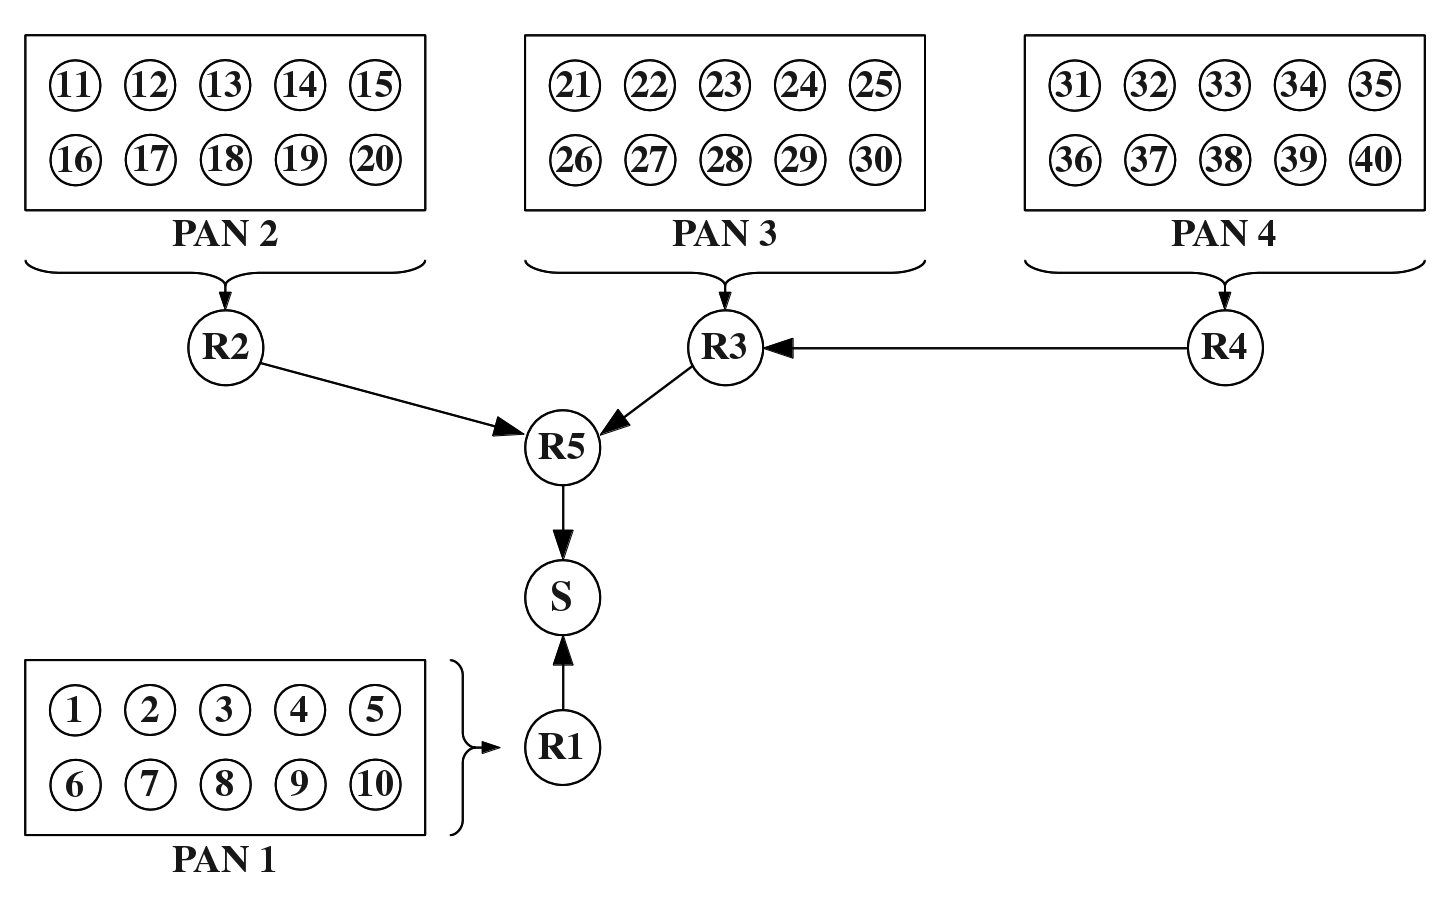
\includegraphics[width=14cm]{images/ch6-config-test-2.png}
\flcaption{Schéma fonctionnel de notre seconde configuration de test.
(Cette topologie est reprise de la publication \cite{iQueueMAC}
en figure 15.)}
\label{FigTestConfig2}
\end{figure}

\end{enumerate}

Concernant le choix des plates-formes, nous avons, comme dit plus haut,
trouvé une opportunité intéressante dans le choix des noeuds IoT-LAB M3
comme nouvelle plate-forme matérielle, notamment pour les performances
nettement supérieures, ainsi que la possibilité de réagir (via des
interruptions) à la détection de SFD par la puce radio, et surtout les
fonctionnalités d'instrumentation avancées (consommation énergétique,
\lang{``sniffer''} de trames radio).

Pour la plate-forme logicielle, nous avons tout naturellement porté notre
choix sur RIOT OS, auquel nous avons déjà participé de façon active, et
qui nous a donné satisfaction dans nos précédents tests par simulation.

%%%%%%%%%%%%%%%%%%%%%%%%%%%%%%%%%%%%%%%%%%%%%%%%%%%%%%%%%%%%%%%%%%%%%%%%%%%%%

\section{Travaux et mise en {\oe}uvre}
\label{SecTravauxMiseOeuvre}


\subsection{Amélioration du pilote radio~: proposition d'API étendue}
\label{SubsecAPIRadioExt}

Afin de commencer nos travaux d'expérimentation sur matériel décrits dans
la section \ref{SubsecTravauxValidPrevus} précédente, il nous a d'abord fallu
nous occuper des couches basses de notre plate-forme logicielle, RIOT OS.

Notre premier travail a concerné le pilote RIOT pour l'émetteur~/ récepteur
radio des noeuds IoT-LAB M3~--- qui pour rappel n'est pas le TI CC2420
comme dans les matériels que nous avions utilisé auparavant, mais
l'Atmel AT86RF231, de conception totalement différente.

Le pilote présent dans RIOT OS au début des présents travaux avec les
noeuds M3 était minimaliste~: il ne permettait que d'envoyer et recevoir
des trames, changer d'adresses et de canal. Il ne permettait ni d'allumer
ni d'éteindre la puce radio, ni de traiter la plupart des exceptions lancées
par cette dernière, et plusieurs bogues empêchaient le fonctionnement correct
lors de l'appel à certains modes avancés (comme l'acquittement automatique
des trames reçues). Nous avons donc dû procéder à des travaux de déboguage
et de complétion du pilote de l'époque. 

De plus, nous y avons ajouté les fonctionnalités nécessaires aux
améliorations algorithmiques dont nous avons parlé par ailleurs dans la
section \vref{SecAmeliorAlgoProtoMAC}, à savoir~: le comptage des SFD
détectés, et la capacité de connaître et définir le seuil (en dBm) à partir
duquel l'émetteur~/ réceptur radio distingue bruit et signal radio utile
(en anglais~: \lang{``CCA Threshold''})~; le tout en prévision de futures
expériences de recherche exploratoire, une fois les travaux de validation
présentés dans la section \ref{SubsecTravauxValidPrevus} précédente
accomplis.

Nous avons pour cela utilisé l'API de <<~capacités~>> dont nous avons
déjà donné le principe en section \vref{ParAPIRadioContiki}. Elle se compose
dans le cas présent de trois fonctions supplémentaires dans l'API du pilote
radio, détaillées en table \vref{TblAPICapFnct}.


\begin{table}[!hbt]
\centering

\begin{tabular}{|l|p{9cm}|}
\hline
\textbf{Nom} & \textbf{Rôle} \\
\hline
\texttt{get\_config\_const()} & Lit la valeur d'une constante liée à la
                                configuration d'une radio donnée~; il s'agit
                                en général d'une limite dictée par le matériel
                                (par exemple~: valeur maximale de la puissance
                                 d'émission en dBm, ou canaux~/ fréquences
                                 radio accessibles) \\
\hline
\texttt{get\_config\_param()} & Lit la valeur courante d'une option de
                                configuration d'un pilote radio donné
                                (par exemple~: nombre de SFD comptés, ou
                                 sensibilité radio en dBm) \\
\hline
\texttt{set\_config\_param()} & Définit la valeur courante d'une option
                                de configuration d'un pilote radio donné \\
\hline
\end{tabular}

\flcaption{Liste des fonctions de l'API complémentaires de <<~capacités~>>.}
\label{TblAPICapFnct}
\end{table}


Nous avons pour nos travaux rajouté seulement deux paramètres, listés en
table \vref{TblAPICapParam}. Notons qu'un nombre arbitraire de constantes et
de paramètres aurait parfaitement pu être rajouté selon les besoins~;
nous nous sommes toutefois limités à ce moment-là au minimum d'ajouts pour
gagner du temps.


\begin{table}[!hbt]
\centering

\begin{tabular}{|l|p{9cm}|}
\hline
\textbf{Nom} & \textbf{Signification} \\
\hline
\texttt{PARAM\_SFD\_COUNT}     & Nombre de SFD comptés par le récepteur
                                 radio depuis son démarrage, ou le dernier
                                 \lang{reset}~; ce paramètre est en effet
                                 remis à zéro pour toute écriture (la valeur
                                 passée à \texttt{set\_config\_param()}
                                 est en effet ignorée) \\
\hline
\texttt{PARAM\_CCA\_THRESHOLD} & Seuil de sensibilité de la radio en dBm,
                                 alias \lang{``CCA Threshold''}~; la puce
                                 radio considère qu'en dessous de cette
                                 intensité, le médium est libre (bruit
                                 résiduel)~; au-delà de cette valeur,
                                 le canal radio est considéré comme
                                 occupé par un signal \\
\hline
\end{tabular}

\flcaption{Liste des paramètres rajoutés par l'API complémentaires de
<<~capacités~>>.}
\label{TblAPICapParam}
\end{table}


Ces fonctions renvoient la valeur voulue (pour les deux fonctions
\texttt{get\_*}), ou une valeur d'erreur parmi celles citées en table
\vref{TblAPICapErr}.


\begin{table}[!hbt]
\centering

\begin{tabular}{|l|p{9cm}|}
\hline
\textbf{Nom} & \textbf{Signification} \\
\hline
\texttt{ERR\_UNKNOWN\_CONST}     & Constante inconnue~/ sans signification
                                   (par exemple~:
                                    \texttt{CONST\_WIND\_SENSE}) \\
\hline
\texttt{ERR\_UNKNOWN\_PARAM}     & Paramètre inconnu~/ sans signification
                                   (par exemple~:
                                    \texttt{PARAM\_CAPTAIN\_AGE}) \\
\hline
\texttt{ERR\_UNAVAILABLE\_CONST} & Constante non supportée par la radio
                                   voulue (par exemple~:
                                   \texttt{CONST\_MIN\_CHANNEL},
                                   constante indiquant le canal minimal
                                   disponible, sur une radio conçue
                                   pour une fréquence unique) \\
\hline
\texttt{ERR\_UNAVAILABLE\_PARAM} & Paramètre non supporté par la radio
                                   voulue (par exemple~:
                                   \texttt{PARAM\_CHANNEL}, paramètre
                                   de choix du canal, sur une radio
                                   conçue pour une fréquence unique) \\
\hline
\texttt{ERR\_READ\_ONLY\_PARAM}  & Tentative d'écriture d'un paramètre
                                   en lecture seule (par exemple~:
                                   \texttt{PARAM\_CURRENT\_ENERGY}, qui
                                   représenterait l'énergie courante sur
                                   le médium radio en dBm) \\
\hline
\texttt{ERR\_WRITE\_ONLY\_PARAM} & Tentative de lecture d'un paramètre
                                   en écriture seule (par exemple~:
                                   \texttt{PARAM\_PERFORM\_RESET}, paramètre
                                   <<~fictif~>> qui réinitialiserait
                                   l'émetteur~/ recepteur radio) \\
\hline
\end{tabular}

\flcaption{Liste des erreurs pouvant être retournées par les fonctions
de l'API complémentaires de <<~capacités~>>.}
\label{TblAPICapErr}
\end{table}


\bigskip

Une fois le pilote RIOT OS pour l'émetteur~/ récepteur radio des noeuds
IoT-LAB M3 prêt, nous avons commencé nos expériences. Ce pilote n'est
par contre pas compatible avec la nouvelle pile réseau RIOT qui a été
présentée dans un chapitre précédent en section \vref{SecGnrcRIOT}
(celle-ci utilise toutefois déjà un mécanisme équivalent, comme nous
l'avons vu). Certaines des idées implantées dans le présent pilote
sont en outre susceptibles, comme nous l'avons également mentionné dans
la section sus-citée, d'être rajoutées (contribuées) à l'API de cette
nouvelle pile <<~gnrc~>>.

\bigskip

Nous avons d'abord réédité notre test de synchronisations entre noeuds
du PAN (cf. section \vref{SecSCoSensRIOTPrecSync}), qui n'a posé aucun
problème~: la précision des synchronisations entre \lang{motes} est
toujours excellente (au niveau de quelques dizaines de microsecondes près).
Le premier des travaux décrits en section \vref{SubsecTravauxValidPrevus}
est donc une réussite.

\bigskip

Nous avons donc ensuite tenté de rééditer notre expérience d'évaluation
de performances (cf. section \vref {SecEvalPerfSCosens}), le second de nos
travaux prévus. De nombreux problèmes techniques complexes et imprévus ont
alors interrompu l'avancée de nos travaux.

Nous allons lister ces problèmes nous ayant empêché d'effectuer les autres
travaux prévus en section \vref{SubsecTravauxValidPrevus}, expliquer la
cause de ceux que nous avons pu résoudre, et donner les éléments que nous
possédons pour tenter de permettre, à l'avenir, la résolution de ceux qui
restent présents.


\subsection{Problèmes techniques rencontrés}
\label{SubsecPbTech}

\subsubsection{Remarques techniques préliminaires}
\label{ParTechnoMote}

Pour permettre de bien comprendre la description des problèmes que nous
allons énumérer, nous allons donner ici quelques détails techniques
d'importance concernant le noeud IoT-LAB M3~--- et surtout ses principaux
composants~: le MCU, l'émetteur~/ récepteur radio, et leur connexion.

\paragraph{Le MCU STM32F103REY.}

Plusieurs détails techniques sont à retenir dans le cas qui nous intéresse~:
\begin{itemize}
\item Ce microcontrôleur, bien qu'étant d'architecture ARM, ne possède
\emph{pas} de MPU (unité de protection mémoire matérielle)~: l'architecture
Cortex-M3 considère en effet la MPU comme une option, que n'a pas retenue
ST-Micro\-electronics pour ce modèle.
\item Comme tous les Cortex-M3, ce MCU possède un NVIC (\lang{Nested
Vectored Interrupt Controller}), un contrôleur d'interruptions avancé
permettant de choisir la priorité des interruptions, le niveau de
masquage, et bien d'autres paramètres.
\item Ce MCU possède de nombreuses GPIO, dont certaines assument également
(selon le mode de configuration) des fonctions annexes~: on citera
notamment les liaisons SPI, I\textsuperscript{2}C, et des UART.
\item Rappelons enfin son espace mémoire~: 512~Ko de mémoire Flash pour
le programme (\lang{``firmware''}) et 64~Ko de RAM pour les données, ce
qui est très confortable.
\end{itemize}

\paragraph{La radio AT86RF231.}

Du point de vue du programmeur, cet émetteur~/ récepteur radio est une
machine à états finis, chaque état représentant une <<~fonction~>> de
la radio. Le graphe des états de cette radio est représenté en figure
\vref{FigEtatsAT86RF231}.

\begin{figure}[!hbt]
\centering
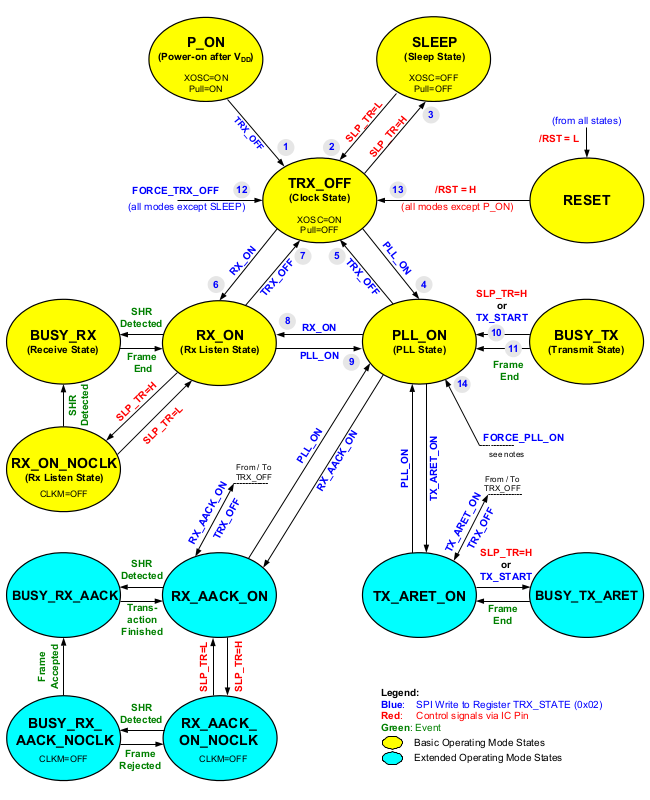
\includegraphics[width=12cm]{images/ch6-etats-at86rf231.png}
\flcaption{Diagramme complet de la machine à états finis de l'AT86RF231.
(Source~: \cite{DSAT86RF231} figure 7-8.)}
\label{FigEtatsAT86RF231}
\end{figure}

Le passage d'un état à l'autre se fait en écrivant dans un registre de
contrôle de la radio (\texttt{TRX\_STATE}), l'état courant étant lisible
dans un registre d'état (\texttt{TRX\_STATUS}). Il s'agit, avec le registre
indiquant les interruptions radio levées (\texttt{IRQ\_STATUS}), des trois
principaux registres avec lesquels travaille le programmeur, l'ensemble
(assez conséquent) des autres registres servant à la configuration
plus <<~stable~>> de la radio (adresse(s), puissance d'émission, etc.)
et étant donc relativement peu lus ou modifiés.

Pour nos travaux, nous avons exploité le mode dit <<~étendu~>> de cette
radio, offrant la gestion automatique de la procédure CSMA~/ CA pour
l'émission (mode \texttt{TX\_ARET}) et l'acquittement automatique des
trames reçus (mode \texttt{RX\_AACK}). Ces modes sont colorés en bleu
dans la figure \vref{FigEtatsAT86RF231}.

Notons également que cette radio peut être mise en mode <<~sommeil~>>
(\texttt{SLEEP}) à très basse consommation, mais que la conception du
noeud IoT-LAB M3 ne permet pas la mise hors-tension totale (\lang{``off''})
de cette puce.

Le mode \texttt{TRX\_OFF} est lui un état où la puce est active, mais
n'accède pas au médium radio ni en émission ni en réception (mode
\lang{``idle''}).

Limitation importante à signaler~: l'AT86RF231 ne possède qu'un \emph{unique
\lang{``buffer''} pour l'émission et la réception}, comme indiqué dans le
chapitre 4 de \cite{DSAT86RF231} (contrairement à d'autres radios comme la
TI CC2420). Des écrasements de données sont donc en théorie possibles si
une trame arrive alors qu'une trame à émettre est en cours de chargement
dans le \lang{``buffer''}~; la radio peut dans ce cas lancer une
interruption d'alerte (\texttt{TRX\_UR}, voir ci-dessous).

\paragraph{La connexion entre MCU et radio.}

Le lien entre ces deux circuits principaux du noeud IoT-LAB M3 est
schématisé en figure \vref{FigLienMCUAT86}.

\begin{figure}[!hbt]
\centering
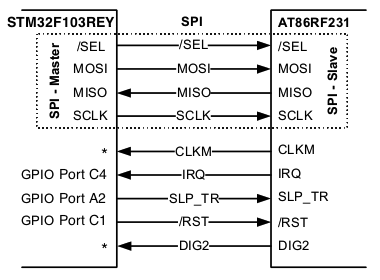
\includegraphics[width=7cm]{images/ch6-lien-mcu-at86rf231.png}
\flcaption{Schéma logique de l'interface entre MCU et AT86RF231 sur une mote
IoT-LAB M3. (D'après \cite{DSAT86RF231} figure 6-1.)}
\label{FigLienMCUAT86}
\end{figure}

Les points importants à retenir de cette liaison sont~:
\begin{itemize}

\item Toutes les communications avec la radio, c'est à dire la lecture
et l'écriture de ses registres, pour configurer et surtout passer d'un
état à l'autre en fonction des besoins, se fait par la liaison SPI.\\
Pour le MCU, il s'agit de la première liaison SPI (correspondant aux broches
4 à 7 du port GPIO A en mode <<~fonction alternative~>>, alias AFIO).\\
Cette liaison SPI est entourée en pointillés dans la figure
\vref{FigLienMCUAT86}, fonctionne de façon standard, et dans notre cas,
est gérée par le pilote générique dédié de RIOT OS.

\item Deux broches GPIO en sortie (du point de vue du MCU) permettent
de déclencher des opérations spéciales~:
  \begin{itemize}
  \item La broche \texttt{RST} (active à l'état bas), permet de réinitialiser
        la radio, par exemple en cas de problème. Elle ramène la puce
        dans l'état \texttt{RESET}, qui transitionne ensuite normalement
        vers l'état \texttt{TRX\_OFF} automatiquement (cf. figure
        \vref{FigEtatsAT86RF231}).\\
        Pour le MCU, il s'agit de la broche 1 du port GPIO C.
  \item La broche \texttt{SLP\_TR} possède deux fonctions, en fonction de
        l'état courant de la radio~:
    \begin{enumerate}
    \item En mode \texttt{TRX\_OFF}, passer \texttt{SLP\_TR} à l'état haut
          met la radio en mode sommeil (\texttt{SLEEP})~; dans ce mode
          sommeil, passer \texttt{SLP\_TR} à l'état bas réactive la radio
          et la ramène en mode \texttt{TRX\_OFF}.
    \item En mode \texttt{PLL\_ON} ou \texttt{TX\_ARET\_ON} passer
          \texttt{SLP\_TR} à l'état haut déclenche l'émission sur le canal
          radio du contenu du \lang{``buffer''}.
    \end{enumerate}
        Pour le MCU, il s'agit de la broche 2 du port GPIO A.
  \end{itemize}

\item Une broche GPIO en entrée (du point de vue du MCU), \texttt{IRQ},
active à l'état haut, permet de signaler au microcontrôleur que la radio
a déclenché une interruption. La broche ne permet pas de savoir de quel
type d'interruption il s'agit~: il est nécessaire de lire (via la liaison
SPI) un registre (\texttt{IRQ\_STATUS}) pour connaître la ou les
interruption(s) déclenchée(s). Notons qu'un autre registre
(\texttt{IRQ\_MASK}) permet d'activer ou désactiver (masquer) le
déclenchement de chaque type d'interruption. Les types d'interruptions
émissibles par l'AT86RF231 sont listées dans la table
\vref{TblIntAT86RF231}.\\
Pour le MCU, il s'agit de la broche 4 du port GPIO C.

\item Nous n'utilisons pas les autres broches de l'interface (\texttt{CLKM},
\texttt{DIG2})~; leur état est toujours ignoré.

\end{itemize}


\begin{table}[!hbt]
\centering

\begin{tabular}{|l|r|p{9cm}|}
\hline
\textbf{Identifiant} & \textbf{No. bit} & \textbf{Description} \\
\hline
\texttt{BAT\_LOW}      & 7 & Indique une chute de tension dans l'alimentation
                             de la radio \\
\hline
\texttt{TRX\_UR}       & 6 & Indique une violation d'accès (écrasement)
                             du \lang{``buffer''} \\
\hline
\texttt{AMI}           & 5 & Si le filtrage d'adresses sources est activé,
                             indique qu'une trame provenant d'une source
                             autorisée à été détecté \\
\hline
\texttt{CCA\_ED\_DONE} & 4 & Si la radio était en mode sommeil ou reset,
                             indique son arrivée en mode \texttt{TRX\_OFF},
                             c-à-d. sa disponibilité~; sinon, indique
                             qu'une procédure de CCA (\lang{``Clear Channel
                             Assessment''}) est achevée \\
\hline
\texttt{TRX\_END}      & 3 & Indique soit la fin de la réception d'une trame
                             (disponible pour analyse dans le
                             \lang{``buffer''}), soit la fin de la
                             transmission de la trame présente dans le
                             \lang{``buffer''} \\
\hline
\texttt{RX\_START}     & 2 & Indique le début de la réception d'une
                             trame (c-à-d. qu'un SFD a été détecté) \\
\hline
\texttt{PLL\_UNLOCK}   & 1 & Indique le déverrouillage de la PLL
                             (condition anormale) \\
\hline
\texttt{PLL\_LOCK}     & 0 & Indique le verrouillage de la PLL
                             (c-à-d. que la radio est prête à accéder
                              au médium radio) \\
\hline
\end{tabular}

\flcaption{Types d'interruptions de l'AT86RF231.
(Source~: \cite{DSAT86RF231} table 6-9.)}
\label{TblIntAT86RF231}
\end{table}


\subsubsection{Détail des problèmes rencontrés}
\label{ParDetailsTech}

\begin{itemize}

\item Des plantages dûs au débordement de la pile système ont eu lieu,
exactement de la même façon que sur les Zolertia Z1, comme nous
l'avons expliqué dans la section \vref{SubsecStabl}. La grande quantité
de RAM présente dans ce MCU Cortex-M3 nous a permis de facilement contourner
le problème en augmentant la taille de la pile à une valeur très élevée
(10~Ko). On peut toutefois regretter l'absence de MPU dans ce
microcontrôleur, étant donné que l'architecture ARM permet d'implanter un
tel mécanisme, qui permet de prévenir efficacement ce type de problèmes.

\item La figure \vref{FigEtatsAT86RF231} montre que l'émetteur~/ récepteur
radio AT86RF231 n'autorise qu'un ensemble bien défini de transitions
autorisées (représentées par des flèches sur la figure sus-citée).
En outre, certaines de ces transitions ne se font pas de façon immédiate,
mais nécessitent un certain délai d'exécution, durant lequel il ne faut
pas tenter de communiquer avec la puce radio via la liaison SPI,
par exemple pour consulter un registre. Ces délais sont (tout comme
l'ensemble des transitions autorisées) précisés dans \cite{DSAT86RF231}.

Par contre, \emph{la même \cite{DSAT86RF231} ne signale pas explicitement
que le non-respect de ces règles peut provoquer la perte du contenu des
registres de l'émetteur~/ récepteur radio, plongeant ce dernier dans un
état de blocage dont seul un RESET peut le sortir}. Cela n'est pas le cas
d'autres émetteurs~/ récepteurs radio, lequels en cas de mauvaise
utilisation signalent une erreur, ou ignorent <<~silencieusement~>>
la manipulation incorrecte, tout en restant capables de continuer
à fonctionner correctement.

La version initiale (préexistante) du pilote que nous avons dû déboguer
effectuait des transitions <<~interdites~>>, ou interagissait avec la
puce radio sans respecter les délais d'attente prescrits~; nous avons
donc fait face à des blocages fréquents de la puce radio, jusqu'à
ce que nous ayons réparé ces erreurs.

Nos corrections ont rendu ce problème beaucoup plus rare. Toutefois,
nous continuons à subir de temps en temps ce problème de <<~remise à zéro~>>
de la puce radio, sans explication logique à l'heure actuelle. 

\item Lors de l'émission de trames, il arrive parfois que la puce radio
n'arrive plus à <<~terminer~>> sa transmission, c'est-à-dire~: revenir
de l'état \texttt{BUSY\_TX\_ARET} à l'état \texttt{TX\_ARET\_ON},
changement d'état normalement automatique une fois l'émission terminée.
Or, l'état \texttt{BUSY\_TX\_ARET} correspond à l'émission d'une trame
en respectant la procédure CSMA~/ CA\footnotemark[3], laquelle comporte
un nombre maximal d'essais et des \lang{``timeouts''} pour éviter de
telles impasses. Nous ne nous expliquons donc pas la raison de ces
blocages... Un RESET de la puce radio est nécessaire pour sortir de ces
situations, qui ne sont heureusement pas systématiques, mais très gênantes,
d'autant plus qu'elles sont actuellement incompréhensibles.

\footnotetext[3]{Revoir dans l'état de l'art la section \vref{ParCSMACA} et
la figure \vref{FigOrganigrammeCSMACA} si nécessaire.}

\item Le problème le plus gênant, car survenant lui \emph{systématiquement},
est le fait que nos noeuds deviennent subitement <<~sourds~>>~: plus
précisément, de façon imprévisible, et apparemment aléatoire, ils deviennent
incapables de recevoir des trames. Ce problème peut apparaître très tôt
durant les expériences, ou survenir après de longues minutes
d'expérimentation. Le MCU n'est pourtant pas planté, car les interruptions
temporelles (du \lang{``timer''} matériel) gérant la génération des trames
se produisent toujours.

\emph{Nous avons découvert que l'interruption chargée de gérer les
évènements en provenance de la puce radio~--- y compris donc les réceptions
de trames~--- ne se déclenchait plus, causant cette <<~surdité~>>.}

\bigskip

Nous remarquons que~:
\begin{itemize}
  \item On note une tendance à avoir des noeuds qui fonctionnent mieux
  que les autres, mais la raison en est inconnue.

\begin{figure}[!p]
\centering
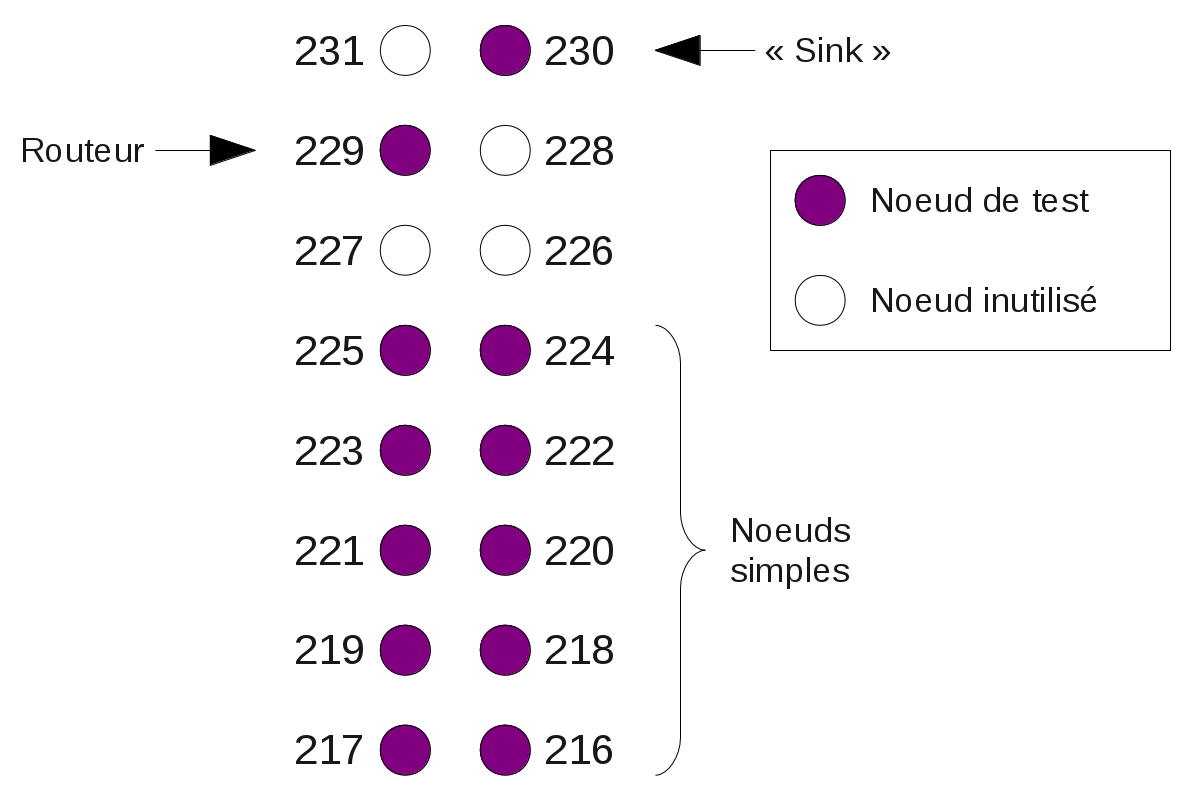
\includegraphics[width=12cm]{images/ch6-disposition-pan-m3.png}
\flcaption{Disposition physique du PAN de test employé sur IoT-LAB
           (noeuds de type M3).}
\label{FigDispoPANM3}
\end{figure}


\begin{table}[!p]
\centering

\begin{tabular}{|l|r|r|r|r|r|r|r|r|r|r|}
\hline
 & \multicolumn{10}{c|}{\textbf{Noeuds}} \\
\hline
 \textbf{Essai} & \textbf{216} & \textbf{217} & \textbf{218} & \textbf{219}
                & \textbf{220} & \textbf{221} & \textbf{222} & \textbf{223}
                & \textbf{224} & \textbf{225} \\
\hline
 I    &  19 &   0 &   0 &  24 & 129 & 287 & 500 &  35 & 500 & 500 \\
 II   &  81 &   0 &   0 & 500 & 500 & 500 & 500 & 211 & 500 &  10 \\
 III  & 500 &   4 &   0 & 500 & 500 & 102 &  17 & 205 & 500 & 500 \\
 IV   & 116 &   0 &   0 & 328 & 500 & 500 & 120 & 114 & 500 & 500 \\
 V    &  49 &   4 &  61 & 500 & 139 & 500 &  97 & 500 & 500 &  91 \\
 VI   &  17 &   6 &   0 & 500 & 500 & 500 &  68 &  66 & 500 &  63 \\
 VII  & 383 &  14 &   0 &   8 & 500 & 500 & 271 &  80 & 500 &  77 \\
 VIII & 500 &   3 &   0 & 500 &  87 & 500 & 105 & 209 & 500 & 209 \\
 IX   & 500 &  21 &   0 & 500 &  17 & 500 &  26 & 478 & 500 & 314 \\
 X    & 500 &   0 &   0 & 500 & 500 & 500 &  89 &  88 & 500 & 500 \\
 XI   & 109 &   1 &   0 & 500 & 500 & 500 & 112 & 107 & 500 & 500 \\
 XII  & 500 &   0 &   0 & 208 & 500 & 500 &  66 &  66 & 500 & 500 \\
 XIII & 500 &  27 &   0 &  23 &  22 & 500 &   7 & 500 & 500 & 500 \\
 XIV  &  25 &   2 &  23 & 208 & 500 & 500 & 500 & 312 & 500 &   9 \\
 XV   & 500 &   0 &   0 & 500 & 309 & 500 & 500 &  33 & 500 &  10 \\
\hline
\end{tabular}

\flcaption{Nombre de trames envoyées avec succès par chaque noeud-feuille,
sur 500 envoyés.}
\label{TblResSCoSenSM3}
\end{table}


  La disposition physique du PAN de noeuds M3 que nous avons utilisé
  (correspondant à la structure logique décrite en \vref{FigVirtualPAN1})
  est présentée en figure \vref{FigDispoPANM3}, les résultats correspondant
  à nos différents essais étant décrits par un échantillon représentatif
  montré en table \vref{TblResSCoSenSM3}.\\
  Cette table montre, comme l'indique sa légende, le nombre de trames
  envoyées avec succès, sur 500 générés au total, par chaque noeud-feuille
  de ce premier PAN de test composé de noeuds IoT-LAB M3.\\
  Au vu de la faible cadence d'envoi~--- 1 trame~/ noeud~/ seconde~---
  il ne devrait y avoir quasiment aucun échec.

  Ces données montrent que la distance entre noeuds et routeur n'a aucune
  influence sur ce manque de fiabilité~: par exemple, le noeud \textbf{224}
  réussit toujours ses envois, et fait donc mieux que le noeud \textbf{225}
  parfois défaillant alors que ce dernier est le plus proche du routeur.
  Même remarque pour les noeuds \textbf{216}, \textbf{217} et \textbf{218},
  le premier (le plus éloigné du routeur) arrivant par intermittence
  à réussir ses envois de 500 trames, alors que les deux autres,
  plus proches, échouent de façon systématique.

  \item Aucune amélioration notable n'est détectable en changeant de
  matériel (c-à-d. de groupe de noeuds pour constituer le PAN de test).

  \item Ce problème survient après un délai apparemment aléatoire
  (il peut survenir immédiatement, ou après l'envoi des trois-quarts
  des trames prévus).

  \item Le blocage des interruptions radio rencontré n'est pas dû à
  une non-sortie (\lang{``deadlock''}) du gestionnaire d'interruptions.
  Des tests avec affichage à l'entrée et à la sortie de ce gestionnaire
  d'interruptions radio ont été effectués~: aucune entrée sans sortie
  n'a jamais été repérée.

  \item Il n'est pas provoqué par un <<~chevauchement~>> d'interruptions~:
  des tests avec blocage des autres interruptions pendant le traitement
  de l'interruption en cours ont été effectués~: aucune amélioration
  constatée.

  \item La table des vecteurs d'interruptions est en mémoire Flash~:
  il est donc impossible que le problème soit lié à un écrasement de
  pointeurs dû par exemple à un débordement de pile (cette dernière piste
  ayant en outre déjà été traitée par une extension majeure de la taille
  de la pile système).

  \item Le problème semble toucher les microcontrôleurs (MCU) des noeuds,
  la broche \texttt{IRQ/C4} des noeuds <<~sourds~>> étant positionnée à 1
  en fin d'expérience, tandis que sur les noeuds <<~sains~>>, cette
  broche est revenue à 0 (puisqu'il n'y a plus rien à recevoir). \\
  Pourtant \emph{aucune différence n'est visible (au bit près) entre la
  configuration physique des MCU des noeuds réussissant à envoyer tous
  leurs trames et ceux <<~devenant sourds~>>}. Sont pourtant vérifiés
  systématiquement, lors de nos comparaisons entre noeuds atteints de
  <<~surdité~>> et noeuds arrivant à recevoir, les registres physiques~:
    \begin{enumerate}
    \item de l'arbre d'horloge, qui alimente bien tous les circuits voulus
          (GPIO, NVIC, EXTI, CPU)~;
    \item des GPIO, notamment du port C4 (qui reçoit la broche \texttt{IRQ}
          de la radio), lequel est bien positionné comme entrée standard~;
    \item du contrôleur d'interruptions~: l'interruption correspondant à
          la broche GPIO C4 (EXTI4) est bien activée, sur front montant, avec
          une priorité suffisamment élevée pour être relayée par le NVIC~;
    \item et de l'unité centrale (CPU) elle-même, c-à-d.~: le c{\oe}ur ARM
          est bien en mode <<~privilégié~>> (nécessaire à l'exécution des
          gestionnaires d'interruptions), et le masquage global de toutes
          les interruptions n'est pas actif.
    \end{enumerate}

  \item L'état de la radio a été affiché régulièrement durant l'éxécution
  (à chaque abandon de l'envoi d'une trame pour cause de file d'envoi
  pleine)~: cette puce radio, lors de périodes de <<~surdité~>>, est dans
  une configuration correcte (mode écoute actif, adresses et canal radio
  corrects, etc.). Ce problème n'est donc pas lié à celui de la <<~perte
  de configuration~>> touchant parfois les puces radio.

  \item Plus la fréquence d'envoi des trames augmente, plus la fiabilité
  diminue~:
    \begin{itemize}
    \item impossible d'avoir 10 noeuds-feuilles fiables simultanément
          à 1 trame~/ seconde chacun~;
    \item impossible d'avoir 2 noeuds-feuilles fiables simultanément
          à 5 trames~/ seconde chacun~;
    \item impossible d'avoir un seul noeud-feuille fiable
          à environ 7 ou 8 trames~/ seconde.
  \end{itemize}
  Cela est étrange, car comme dit au point précédent, la configuration de la
  puce radio ne montre dans ces cas-là aucune anomalie.\\
  Plus encore, l'AT86RF231 dispose d'une fonctionnalité étendue nommée
  \lang{``High Data Rate Modes''} (voir \cite{DSAT86RF231} section 11.3),
  lui permettant d'émettre et de recevoir à un débit pouvant monter jusqu'à
  2000~Kb/s (\emph{huit fois} le débit nominal IEEE 802.15.4) au prix d'une
  sensibilité diminuée ($-89$~dBm au lieu de $-101$~dBm en mode IEEE 802.15.4
  standard). Même si nous n'utilisons absolument pas ces modes à haut débit,
  il semble difficilement crédible qu'un composant, capable de dépasser aussi
  largement les limites de débit du standard, se bloque lorsque cette
  limite officielle de base de 250~Kb/s est approchée...

  \end{itemize}

\end{itemize}

\subsubsection{Résumé~: les problèmes rencontrés et leur traitement}
\label{ResumePbTech}

Nous avons recherché les causes de ce problème aussi bien au niveau
logiciel (plus précisément~: dans notre code), qu'au niveau de la radio ou
du microcontrôleur lui-même. Mais comme nous l'avons dit, nous avons vérifié
la configuration de la puce radio de façon poussée sans résultat.
Concernant le MCU, nous avons examiné la configuration des entrées~/ sorties
(GPIOs et AFIOs), des interruptions et évènements (NVIC et EXTI), de l'arbre
d'horloge (RCC) \cite{ManSTM32F10x}, et du c{\oe}ur ARM Cortex-M3 lui-même
\cite{ManSTMCortexM3}, sans trouver d'explication logique quant à cette
désactivation de l'interruption liée à la radio, ni aucune piste valide
quant à sa ou ses cause(s). Nous avons également longuement et
soigneusement testé et modifié notre code, en vain.

\medskip

\`A l'heure actuelle, trois possibilités nous viennent à l'esprit
pour expliquer ce phénomène~:
\begin{itemize}
\item Nous pouvons nous demander si une défaillance brève mais marquée
dans l'alimentation des noeuds (en anglais~: \lang{``brownout''}) pourrait
provoquer ces problèmes. Certains éléments font penser à une telle
hypothèse, mais nous n'avons aucun moyen de la vérifier, ce MCU ne
comportant pas de mécanisme de détection de \lang{``brownout''} comme
en ont d'autres microcontrôleurs~--- ni même un mécanisme basique de
contrôle de la tension d'alimentation comme la radio AT86RF231
avec son interruption \texttt{BAT\_LOW}.\\
Notons toutefois que la baisse de fiabilité corrélée au débit des
trames, quel que soit le nombre de noeuds, semble contredire cette
hypothèse~; sauf si tous les noeuds employés lors de nos expériences
dépendent de la même alimentation.
\item Nous pouvons soupçonner un problème dans le mécanisme de gestion
des interruptions dans le noyau de RIOT. Mais dans ce cas, pourquoi
l'interruption liée à la radio est-elle la seule touchée~? Nous savons
que les timers matériels (qui correspondent à un autre type d'interruption)
restent eux fonctionnels sur tous les noeuds, y compris ceux touchés par
le problème. En outre, après avoir signalé le problème sur les listes
de diffusion de RIOT, aucun autre utilisateur ne semble rencontrer la
même situation.
\item Nous pouvons penser qu'un autre circuit appartenant au microcontrôleur,
outre ceux dont nous avons vérifié les registres matériels, est parfois mal
configuré. Toutefois, vu l'étendue des sous-systèmes du MCU dont nous avons
vérifié les registres, nous ne voyons absolument pas quelle autre partie du
microcontrôleur serait susceptible de provoquer de telles anomalies.
\end{itemize}
Comme on le voit, aucune de ces trois hypothèses n'est vérifiable facilement,
ni suffisante à elle seule pour pouvoir expliquer toutes les anomalies
constatées.

Nous n'avons en résumé aucune piste solide quant à la cause des
problèmes que nous rencontrons, ni par conséquent du moyen de les
résoudre ou même de les contourner dans le cadre de cette thèse.


\subsection{Situation actuelle}
\label{SubsecEtatActuel}

Nos dernières expériences sur les noeuds IoT-LAB M3 ont toutes échoué~---
impossible d'avoir des résultats fiables~--- à cause de ce problème de
<<~surdité~>> des noeuds.

Ce problème étant comme nous l'avons dit systématique, aucune expérience
n'arrive à son terme sans erreur~: tenter de les multiplier dans le but
d'obtenir assez de résultats réussis sur le long terme est inutile.

En outre, d'autres problèmes rencontrés surviennent encore de façon
sporadique~:
\begin{itemize}
\item perte de sa configuration par le transmetteur radio, ce qui oblige
à redémarrer le noeud touché~;
\item problème de non-sortie du mode de transmission d'un trame.
\end{itemize}

Là également, nous ignorons les causes de ces anomalies.

\medskip

Quelques discussions avec les ingénieurs du projet IoT-LAB nous ont appris
que la plate-forme logicielle de référence sur les noeuds IoT-LAB M3 n'est
pas RIOT OS, mais OpenLab d'HiKoB (la société ayant conçu ces matériels),
ce qui explique que peu d'utilisateurs d'IoT-LAB soient concernés par
ce problème, et~/ ou en mesure de nous aider.

\bigskip

Comme indiqué dans la section \ref{ResumePbTech} précédente, nous n'avons,
malgré nos nombreux efforts, actuellement trouvé aucune piste technique
significative pour expliquer, contourner ou résoudre ces problèmes.

Ce problème a vraisemblablement une cause complexe (voire plusieurs causes
multiples), tout comme celui qui touchait le portage de RIOT OS sur MSP430
\cite{PRriotFix1MSP430} \cite{PRriotFix2MSP430} \cite{PRriotFix3MSP430}.
Toutefois, nous sommes ici face à un appareillage d'un niveau de complexité
bien supérieur à celui d'un noyau MSP430.

Corriger le ou les bogues sous-jacent(s) qui provoque(nt) les problèmes
auxquels nous faisons face est évidemment un travail de longue haleine,
dont la durée peut difficilement être estimée précisément~--- mais se
compterait probablement en mois, pour reprendre l'exemple antérieur de RIOT
sur MSP430. Il s'agira en tout cas d'un travail d'ingénierie de haut niveau,
nécessitant clairement du personnel compétent et formé, sinon aux WSN,
du moins aux systèmes embarqués.

Pour toutes ces raisons, nous n'avons donc pu réaliser que le premier des
travaux envisagés en section \vref{SubsecTravauxValidPrevus} en temps voulu.

Nous espérons qu'un travail ultérieur à cette thèse permettra de résoudre
ces problèmes~--- ou de passer outre, par exemple en employant une autre
plate-forme matérielle~; à moins que la nouvelle pile réseau de RIOT, que
nous avons abordé dans la section \ref{SecGnrcRIOT}, ne permette, même
partiellement, de régler ces difficultés~--- et en tirera les bénéfices
et contributions pour l'instant manquants que nous citons en section
\vref{SubsecTravauxValidPrevus}.

Nous souhaitons également que les informations techniques et pistes de
réflexion que nous avons compilées dans la présente section contribuent
à la découverte d'une future solution à ces différents problèmes techniques.

\medskip

Enfin, notons que des travaux sont d'ores et déjà en cours pour tenter de
porter nos protocoles MAC~/ RDC avancés sur la nouvelle pile <<~gnrc~>> de
RIOT OS, afin de pouvoir tester dès que possible si cette dernière permet 
d'apporter des avancées concernant ces difficultés (voir section
\vref{SubsecPerspCourt} sur les perspectives à court terme).

%%%%%%%%%%%%%%%%%%%%%%%%%%%%%%%%%%%%%%%%%%%%%%%%%%%%%%%%%%%%%%%%%%%%%%%%%%%%%

\section[Discussion~: validation, contributions et conclusion]
        {Discussion~: validation des expérimentations, contributions
         et conclusion}
\label{SecConcluChValidation}

Nous avons dans le présent chapitre \emph{apporté les contributions
suivantes}~:

\begin{itemize}

\item Nous avons clairement montré que \emph{l'émulation effectuée par le
logiciel MSPSim souffre d'un sérieux problème d'inexactitudes temporelles
concernant l'accès au bus SPI, probablement dû à une mauvaise calibration
des délais pour l'émulation des MCUs}. Ce problème impacte les
communications entre les microcontrôleurs et les émetteurs~/ récepteurs
radio~--- et par conséquent, les opérations liées à la radio~--- dans les
\lang{motes} constituant les réseaux de capteurs sans fil.

\item Nous avons \emph{décrit la gravité du problème avec des résultats
d'expérimentations détaillées}~--- gravité qui se trouve être sérieuse,
tout spécialement concernant l'émulation de la plate-forme matérielle
Zolertia Z1.

\item Nous avons \emph{fourni des pistes sérieuses quant aux causes de ce
problème}, et par conséquent délimité une zone raisonnable d'investigation
à traiter pour parvenir à une correction des erreurs sous-jacentes et
à une résolution de ces difficultés.

\item Nous avons \emph{proposé une extension générique de l'API des pilotes
radio (couche 1) des piles réseau des plates-formes logicielles spécialisées
dans les WSN}. Si notre première implantation décrite dans ce chapitre
ne pourra pas être réutilisée, cette idée à d'ores et déjà été reprise
et implantée par RIOT OS (comme nous l'avons vu précédemment en section
\vref{SecGnrcRIOT}) et Contiki dans sa version 3.0 (partiellement et
indirectement grâce à nos contributions). Nous sommes en outre convaincus
que \emph{cette API générique, à la fois simple et performante, peut être
adaptée à toute plate-forme logicielle, et même à toute pile réseau, pour
améliorer l'interface de ses pilotes radio} (interface entre la couche 1
et les couches supérieures) dans le domaine des WSN, et certainement
même dans un cadre encore bien plus général~: on peut comparer notre
concept à la primitive \texttt{ioctl()} classique dans le monde
Linux/Unix/POSIX).

\item Nous avons \emph{proposé une liste de travaux devant permettre de
valider nos précédentes expériences avec S-CoSenS, puis tester la <<~montée
en charge~>> de ce dernier sur un réseau étendu reproduisant assez
fidèlement le niveau de complexité d'un <<~logement intelligent~>>},
qui représente le principal domaine d'application du contexte de la présente
thèse (le projet LAR).

\medskip

\item Malheureusement, des problèmes techniques que nous n'avons pu résoudre
nous ont empêché de mener les dits travaux à leur terme. Nous avons alors
\emph{fourni le maximum de détail techniques concernant les problèmes
recontrés et les plates-formes sous-jacentes, dans l'espoir de faciliter
la résolution de ces difficultés et le succès des travaux que nous avions
prévus lors d'un travail ultérieur à la présente thèse}. Notons que nos
investigations nous font penser que ces problèmes sont complexes,
potentiellement provoqués par plusieurs causes distinctes, et que
leur résolution représentera un travail d'ingénierie délicat et donc
potentiellement long à accomplir.

\end{itemize}

\bigskip

Ce chapitre aura au final démontré la fragilité des résultats d'expériences
obtenus par simulation~/ émulation~: si ceux-ci sont bien plus faciles et
moins coûteux à obtenir~--- surtout en quantité et avec les éléments de
précision désirés~---, ils sont toujours susceptibles d'être faussés par
des inexactitudes ou des erreurs dans les logiciels de simulation ou
d'émulation, comme nous venons de le voir pour le \lang{framework} Cooja~/
MSPSim. Le recours abondant à ces techniques de simulation~/ émulation
pour évaluer des travaux dans la littérature pousse à se poser des questions
quand à la validité de nombreuses publications.

Soulignons néanmoins que ces outils de simulation et d'émulation sont par
contre de formidables outils de développement et de déboguage, simplifiant
souvent, et parfois considérablement, ces deux tâches. Ces fonctionnalités
suffisent à elles seules à justifier l'existence et le développement continu
de tels outils logiciels.

\medskip

L'évaluation fiable du fonctionnement de réseaux sans-fil, et en particulier
de projets conçus sur la technologie des WSN, nécessite \lang{a contrario}
le recours à des tests sur matériel réel, comme nous pensons l'avoir
démontré ici. La mise en place de tels tests n'est en aucun cas triviale~:
elle est longue, coûteuse, et présente des difficultés techniques nombreuses
et souvent difficiles à résoudre~--- plus que l'on ne l'imagine en général
au premier abord.

Des efforts ont été mis en place pour faciliter l'exécution de tels tests,
comme le \lang{testbed} Iot-LAB, que nous avons longuement utilisé et
décrit dans le présent chapitre. Malgré tout, nous avons pu voir que
malgré les moyens importants déployés par ce projet~--- notamment en
matériels et compétences humaines (ingénieurs du projet réactifs et
disponibles pour aider les utilisateurs)~--- nous n'avons pu surmonter
les problèmes techniques qui ont interrompu nos travaux de validation.
Les difficultés qui entravent les tests de validation d'expérimentation
sur matériel concernant les WSN sont donc bien réelles, importantes, et
ne sauraient être sous-estimées. Cela explique aussi sans doute aussi
pourquoi les validations par simulation~/ émulation sont encore souvent
employées~: par défaut.

\bigskip

Au final, ce chapitre, s'il n'a pas, comme nous l'escomptions, validé nos
précédentes expérimentations sur S-CoSenS, se révèle être riche en
enseignements, parfois désagréables à constater, et représente~--- nous
l'espérons~--- une source de renseignements qui permettra la poursuite de
nos travaux de validation dans un travail ultérieur, et au mieux fournira
explications et solutions pour faciliter d'autres futurs travaux
d'expérimentations de WSN sur matériel réel. Il d'agit donc là de
perspectives à court mais aussi peut-être à plus long terme, que nous allons
détailler dans le chapitre \ref{ChConcluPerspec} suivant, après
les conclusions générales de ce manuscrit.


%%%%%%%%%%%%%%%%%%%%%%%%%%%%%%%%%%%%%%%%%%%%%%%%%%%%%%%%%%%%%%%%%%%%%%%%%%%%%
%%%  FIN DU CHAPITRE "VALIDATION EXPÉRIMENTATIONS / TESTS SUR MATÉRIEL"   %%%
%%%%%%%%%%%%%%%%%%%%%%%%%%%%%%%%%%%%%%%%%%%%%%%%%%%%%%%%%%%%%%%%%%%%%%%%%%%%%

